\documentclass{article} 

\usepackage{graphicx}
\usepackage{subcaption}
\usepackage{multirow}
\usepackage{amsmath}
\usepackage{hyperref}

\begin{document}

\section*{Acknowledgements}
I would like to thank my supervisor Dr. Aphrodite Galata for her commitment to the project and her generous advice on my progress throughput the year. Also, I would like to thank my parents for backing me up and help me cope with lots of things that I shall spend much time on.
\newpage

\section*{Abstract}
In this project I aimed to build a program for tracking players in broadcast football video. Due to the complexity of the topic, the project mainly focused on videos from static camera, but keeps the potential to extend to those from rotating camera. The whole program can be divided into 4 parts: player detection, player identification, tracking and label correction. 
The program is based on a set of python scripts. A pretrained model produced by Mask-RCNN is used for player detection, SIFT features from MSERs of each detection are put into BOVW model and KNN is used for classification of BOVW features. Idea of tracking-by -detection is used in tracking part, and a tracklet is maintained for each player. Kalman filter is used here to give more robust tracking and do prediction of player locations where occlusions occur. A simple majority label assignment is done for label correction part.
\newpage

\tableofcontents
\newpage
\listoffigures
\newpage
\listoftables
\newpage

\section{Introduction}
Figure tracking has been a widely investigated problem and there are many satisfying results for pedestrian tracking. However, research of tracking for sports players is not that well extended as it is more difficult due to unpredictable trajectories. Low quality of players also poses a challenge, as it limits number of features of each figure and brings difficulty to identification.\\
This report will describe current milestone and strengths \& weaknesses of the system. Relevant work of previous students[1][2] provides some reference on methodology and further discoveries have been made. Evaluation will be done on player detection and identification. In the report, part 2 will describe previous works on the field of tracking sports players as a whole and relevant technologies on each part of system; part 3 states methods I worked on for each of 4 parts of the system, part 4 includes procedure of evaluations I mentioned above and gives their results, finally, strengths and weaknesses of my final work will be discussed in part5. 
\subsection{Aim}
An ideal version of the project is a system that can generate tactics automatically, yet this includes translate players’ identities and trajectories into strategies, thus being way too complex for the given amount of time and will need participation of football professionals. For this project, the system is expected to generate a bounding box for every player in each frame and a correct and consistent identity should be given to each figure across the frames he/she appears in the video.
\subsection{Challenges}
A list of different challenges needed to be overcome is listed below.
\begin{itemize}
\item 1. Unlike pedestrian tracking, which give close and clear image of people, the camera for a broadcast sports video is usually placed relatively far from players and thus people in result videos usually have smaller size and keep less detail. This presents difficulty for both identification and identification, as limited information can be utilized. Apart from that, players in broadcast usually moves at a variant speed and unpredictable direction, posing challenge to detection and tracking. When players move at high speed, they usually look blurred in the video, making identification harder.
\item 2. All players in a team wear the same kind of jersey, making individual player classification become difficult. 
\item 3. Distinguishability of players depends on many factors, like lighting condition of the scene, whether color of players’ jersey and background are similar, etc.
\item 4. Using only one camera will cause problem of occlusion occurs frequently. Information of a player will get lost completely as long as he/she is occluded, causing difficulty to maintain continuity of tracking.
\end{itemize}
\subsection{Approaches}
Going directly to a broadcast video of a real match is a step way too big, a reasonable baseline will be trying various kinds of methods on a simplified scene, like the dataset I am provided that includes only 4 players instead of 22. Satisfying results on such simple scenes will make it convincible that the same method has potential to work on a more complex video, otherwise it shall be abandoned.\\
(screenshot: occlusion, moving at high speed, dim background, jersey same color with background)
Python is used for the whole project, mainly for 3 reasons:
\begin{itemize}
\item 1. It provides various kinds of commonly used data structures like list and dictionary;
\item 2. A large number of packages are available for python, getting me avoid of building many things from scratch.
\item 3. Taking into the account of usage of deep learning framework, python is the best choice as almost all frameworks provides the best-written, most informative documentation only for python, python frameworks has been most wide used by other deep learning workers, with more bugs fixed, more problems discussed, being more robust, thus will cause less problem when I integrate a neural network model in the project.
\end{itemize}
\subsection{Impact of COVID-19}
By the 
\newpage

\section{Background}
The topic of sportsperson tracking is still an ongoing one and a considerable part of work is about investigation into if tracking in low-quality sports video is achievable. In this section, previous works on this topic are introduced first, then for player detection, player identification and tracking, algorithms and ideas I tried on are briefly explained.
\subsection{Previous work}
Work of Lu \textit{et al.}[3] is where I get a majority of ideas to build my system. They used a Deformable Parts Model to detect players. SIFT features, MSER regions and color histogram are used represent players in classification task. Idea of tracking-by-detection is used in tracking part with Kalman Filter for player state estimation. Finally, Conditional Random Field is integrated into their work for performing joint classification, allowing them to borrow statistical strength from the reliable classifications to help ambiguous classifications.\\
Beetz \textit{et al.}[4] built the system ASPOGAMO(Automated SPOrt Game Analysis MOdel) for football player tracking. It can give results of player detection and their traces and has the ability of working real-time. By estimating camera parameters, the system map location of players in a frame to their co-ordinations in a pitch. A color model is built for each type of players and template matching is used to localize location of players. Each model then forms a template and scan across the whole frame to detect and identify players at the same time. Classified detections are then put into Multiple Hypothesis Tracker for tracking task.\\
In work of Liu \textit{et al.}[5]detection work is done by boosted cascade detector trained on Haar features, aided by background region filtering after the its color is learned. A player appearance model, built on GMM with bag of features representing players, is utilized to do classification. Tracking is regarded as a data association problem with the help of MCMC strategy.\\
Previous students [1] and [2] --basically work of [2] is based on [1] --tried background subtraction and linear SVM detector based on HOG feature for player detection, KNN based on BOVW features for classification and idea of tracking-by-detection with support of Kalman Filter for tracking. [2] also used CRF for label correction mentioned in [3], yet the author build a CRF per tracklet and did not utilize the mutex relation among tracklets, so it can be roughly regarded as using a majority label assignment.\\
He \textit{et al.} [6] proposed Mask-RCNN network architecture for generic object detection, which has satisfying performance on detection of person and being one of the most state-of-the-art networks for object detection task.\\
Recently a survey [7] is published on various kinds of methods for sportsperson tracking, in which challenges and ways to mitigate them are briefly introduced. Unpredictability of players’ movement is seen as an obvious challenge, yet some researchers managed to mitigate its impact by predicting players’ locations in advance. Occlusion is another issue and a possible solution of using multiple cameras is provided.\\
Given that broadcast from single camera is used in the project, I first tried out the detection method used in [1] and [2], yet later migrate to using a pre-trained model from Mask-RCNN network. In identification phase, I utilized idea given in [3]. My approach for tracking is borrowed from the work of [3] and for label correction a method of majority label assignment is used after seeing the plausibility analysis of CRF on all tracklets in [3] and Actual effect of the simplified version of CRF used in [2].
\subsection{Player detection}
To do player tracking, we first need to know where they are. For videos from static cameras locating is relatively not that difficult, yet such kind of videos are too rare, especially in popular sports like football and basketball, so techniques suitable for moving scenes are later considered. \\
Machine learning with explicit features is likely to cope with the problem, deep learning with implicit features may also be a choice, as there are lot of successful experiences of applying both of them to general object detections.
\subsubsection{Background Subtraction}
Background subtraction is a technique that removes all backgrounds in the image, leaving only the foreground. Here background means whatever we are not interested in.\\
\begin{figure}
  \centering
  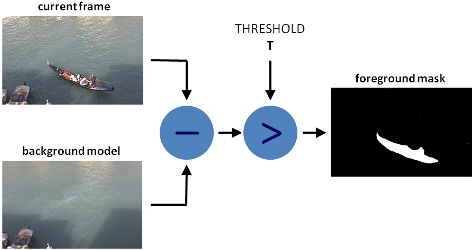
\includegraphics[scale=0.9]{report/pic/2/Background_Subtraction_Tutorial_Scheme.png} 
  \caption{Procedure of background subtraction}
\end{figure}
By saying ‘subtraction’, we can easily think of the most direct and literal way of doing this: doing difference between images. Ideally, background won’t change across frames. So as long as we have an initial frame of background image and any other frame, we can simply isolate fore ground by subtracting pixels at the same position. Those represent background of course will not change and difference result will be 0, and for pixels occupied by foreground it shall be non-zero. Then simply applying a threshold to the difference image can give us the binary image, where zeros are backgrounds and ones are foregrounds.\\
However, we can seldom acquire a completely static background due to brightness change and wind disruptions to camera, meaning that background shall constantly be at slight change. This requires us to continuously update our background, or changed background will be misclassified as foreground, becomes noises in final binary image, and causing difficulty when we try to identify true foreground.
One way of doing this is using Gaussian Mixture Model(GMM), suggested by Friedman and Russell [8]. By adapting such a technique, we assume however the color of background model change, its value shall fall into a combination of Gaussian clusters that together represents the model. We try to do a binary classification on every pixel to determine whether it belongs to background or not.\\
Given a footage, the first frame is assumed to be the background image and used to build the GMM. As a new frame comes, every pixel will be classified and acquired background will be used to update the model, and this new  background will then be subtracted from the next frame later. In this way,  background is kept up-to-date and historical data older than a threshold will be discarded. 
In the context of player detection, obviously players should be regarded as foreground and they should be extracted easily as they are always moving, unlike (almost) static background. However, it should be also noticed that there is also a moving ball in the frame, so additional methods should be used to filter out its blob.\\
\subsubsection{Detection by model based on HOG features}
A feature descriptor is some useful data extracted from an image that has actual meaning and can somehow represent the image. Among various kinds of feature descriptors, Histogram of oriented gradients (HOG), introduced by Dalal and Triggs [9], is widely applied to human detection.\\
\begin{figure}
  \centering
  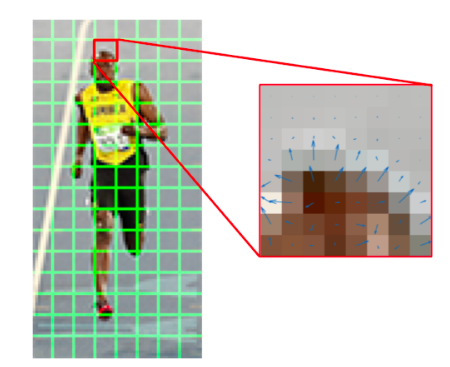
\includegraphics[scale=0.5]{report/pic/2/Sample_of_gradients.png}
  \caption{A heuristic view of gradients in a cell}
\end{figure}
\begin{figure}
  \centering
  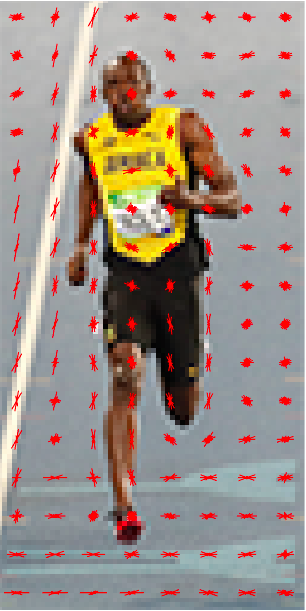
\includegraphics[scale=0.3]{report/pic/2/HOG_of_a_picture.png} 
  \caption{HOG of a detection window}
\end{figure}
For each cell that a picture is divided into, image gradients re calculated upon it. The gradients of adjacent cells (called blocks) are then grouped into HOGs and HOGs for each block of the picture eventually form the HOG\ feature of the picture. An SVM classifier can then be trained to do detection work according to the features of positive and negative samples, like the inventors of HOG did in [9]. For actual detection, a sliding window will go through the target picture and the cropped image captured by this window is put into SVM for detection.

\subsubsection{Detection by pre-trained model from Mask-RCNN}
Instead of extracting features explicitly, a Convolutional Neural Network (CNN) picks information from pictures in implicit ways. Due to its convenience of adding non-linearity to models simply by adding activation functions, it gains extraordinary power of doing detection, segmentation and classification task and has become a popular, if not the first, candidate when dealing with images.\\
\begin{figure}
  \centering
  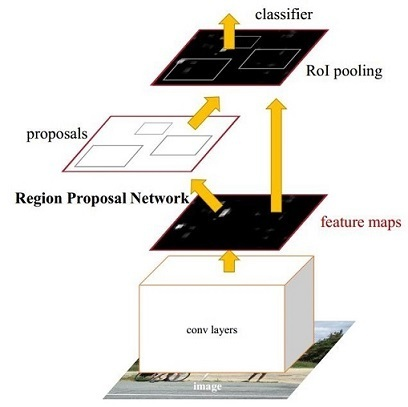
\includegraphics[scale=0.5]{report/pic/2/RCNN_arch.jpg} 
  \caption{Architecture of Faster-RCNN}
\end{figure}
Through years of evolution CNN acquires larger power of instance segmentation (object detection \& instance segmentation). By now the most state-of-the-art product is Mask-RCNN. For object detection it used a sub-architecture similar to Faster-RCNN, and for instance segmentation a Fully Convolutional Network (FCN) is utilized. Since only the detection part is what we want, we focus on the Faster-RCNN-like part.\\
Instead of getting a window swept across the whole picture, which is clearly non-efficient, a pretrained Region Proposal Network(RPN) is used to generate possible bounding boxes on feature maps.\\
\begin{figure}
  \centering
  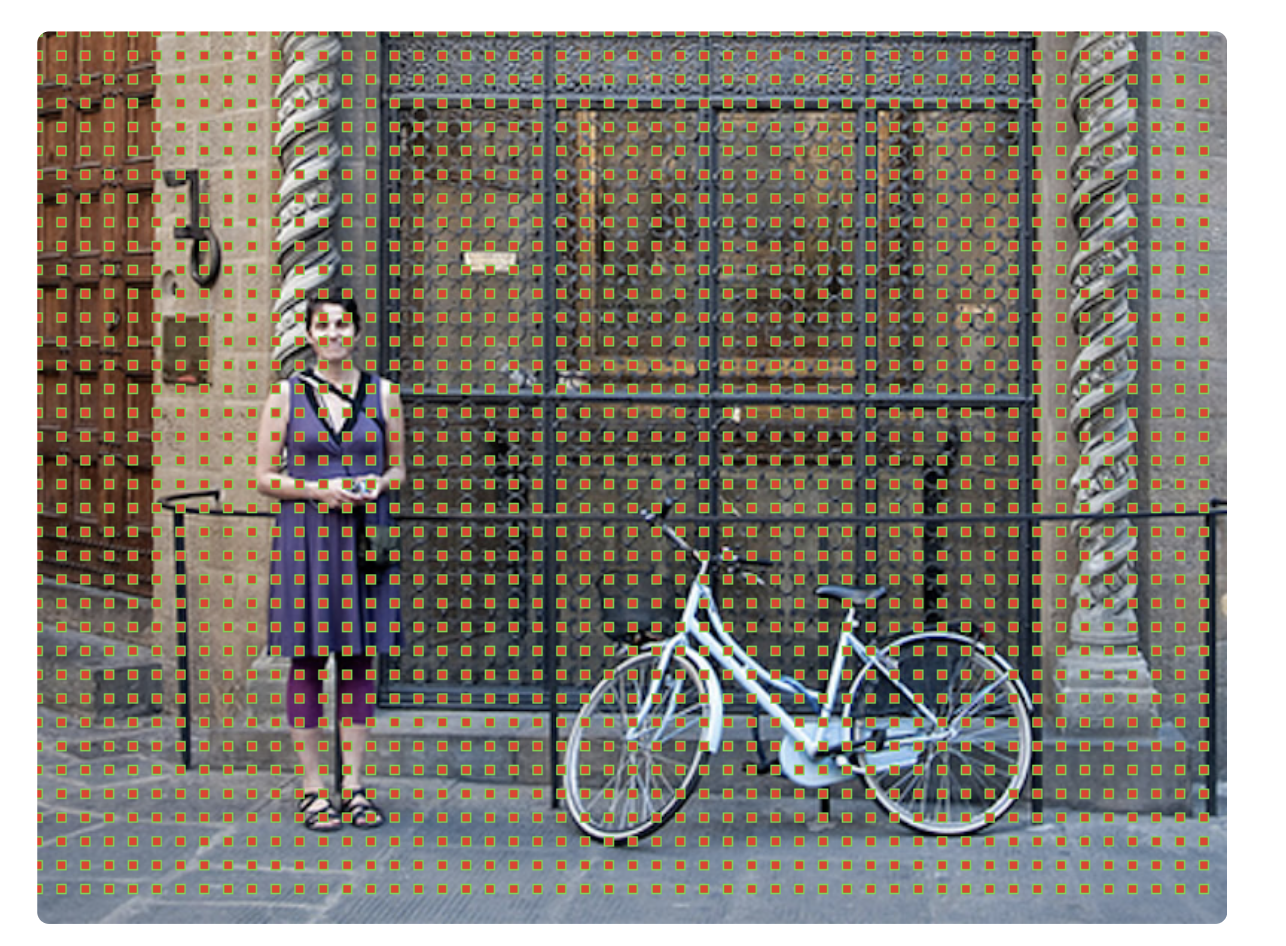
\includegraphics[scale=0.25]{report/pic/2/anchor_point.png} 
  \caption{An picture with anchor points}
\end{figure}
In RPN, each point in feature map is mapped back to corresponding locations as anchor points. 9 boxes of different sizes on each anchor point is generated to check if there is any object. Bounding box regression is then done on boxes with objects. It is used to adjust shape and position of bounding box so as to get it contain the whole object rather than just part of it. This can be done at testing phase because at training phase the dissimilarity between generated bounding box and ground truth bounding box is added to the loss function to get it minimized. Non-maximum suppression is then applied to discard boxes with high IoU score.\\
Now that refined boxes are produced by RPN, they are then used to pool features from feature map, done by pooling layers. There are some fully-connected layers for flattening.\\
Output of fully-connected layers will go into 2 branches, one for classification, the other for further bounding box regression. Unlike that in RPN where regression is done on all boxes uniformly, here the regression function depends on classification result; in other word, boxes for different kinds of object object will be regresed in different ways.\\
FInal output will be a picture with bounding boxes, each box with a label accompanied as a result of classifcation.\\
\subsection{Player Classification}
After detections are obtained, players picked out still needs to be classified to give their identification and to get their information updated correctly during tracking. In broadcast videos, face detection is not feasible due to low resolution and sometimes blurs during moving, so more salient and scale \& rotation-resistant features should be chosen.
\subsubsection{Features}
\paragraph{4.3.1.1 RGB histogram}
As human we mostly distinguish one person from another by different colors of clothes they wear, and computer may also borrow the knowledge of color for classification.  Using raw color values may not be a plausible as this may cause our vectors to include similar features like a darker blue or a slightly brighter one. Similar feature does no help but adds to computational burden, so we use RGB histogram instead. For each color channel, a range of values are put into one bin, and a histogram represents occurrence frequency of colors in different value ranges. This histogram can then be used as (a part of) feature vector for classification.
\paragraph{2.3.1.2 SIFT}
Players are always moving. They appear smaller in a frame when being far from camera and gets larger when getting close; directions they face are always changing and they are continuously in different poses. Despite that we still want to classify “detection of plater A” as “player A” however he/she looks in the video, so a feature that is invariant towards scale and rotation shall be used/integrated. Scale-invariant feature transform (SIFT), proposed by Lowe[11], meets this requirement. It has 4 major steps:
\begin{figure}
  \centering
  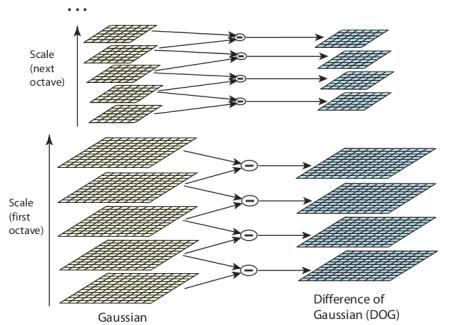
\includegraphics[scale=0.5]{report/pic/2/sift_dog.jpg} 
  \caption{Doing DoG on adjacent $\delta$ s.}
\end{figure}
\begin{figure}
  \centering
  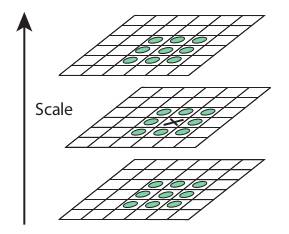
\includegraphics[scale=0.5]{report/pic/2/sift_local_extrema.jpg} 
  \caption{Finding local extrema.}
\end{figure}
\begin{itemize}
\item 1. Scale-space extrema detection: The difference of Gaussians function is used to efficiently search the image and find potential keypoints. Gaussian blur filters are applied across a range of scales, and the differences between adjacent images are computed to create difference images. Local minima and maxima in the difference images are noted as potential keypoints, found by comparing each pixel to the eight neighbors in the same image and nine neighbors in both adjacent images.
\item 2. Keypoint localization: Candidate keypoints are filtered to find those invariant to scale and orientation. Edge responses and keypoints with low contrast are removed. Locations are refined by using data from neighboring scales to find the most suitable scale.
\item 3. Orientation assignment: A histogram of oriented gradients is computed over the neighborhood of each keypoint, with 36 bins to cover 360. The bin with the highest peak is picked as the dominant orientation, and the patch is normalized by this so that all future calculations are done with respect to this orientation.
\item 4. Keypoint descriptors: The patch surrounding the keypoint is divided into 16 cells (4 by 4 sub-patches), and a histogram of oriented gradients with 8 bins is calculated for each cell (Figure 8). These are concatenated to form one vector of length 128 (16 cells ⇤ 8 bins) used to represent the patch.
\end{itemize}
\subsubsection{BOVW}
\begin{figure}
  \centering
  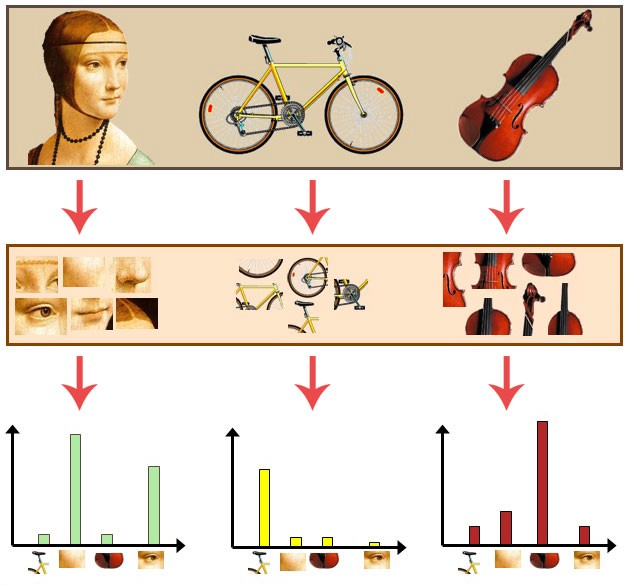
\includegraphics[scale=0.4]{report/pic/2/build_BOVW_histogram.jpeg} 
  \caption{Build BOVW histogram.}
\end{figure}
\paragraph{2.1.3.3 MSER}
Maximally stable extremal regions (MSERs) are regions that are connected components that keep its shape unchanged throughout appliance of a range of thresholds. Intuitively, these regions we get will have their color obviously different from their surroundings, thus should be considered regions of interest (ROI). In work of [3], SIFT features are extracted from MSERs of a detection.
Bag Of Visual Words (BOVW) model originates from field of NLP, trying to represent an image with a set of ‘visual words’. In [3], SIFT from MSERs are not directly used for classification, but first grouped into visual words, then visual word histogram (occurrence frequency) is used as feature of vector for an image. This is done for 2 reasons:
\begin{itemize}
\item 1. number of SIFT extracted from every image is different. As we all know features should have the same length first to put into classifiers, so their length should be normalized in some way.
\item 2. some SIFT in an image may represent similar features and it is unnecessary to see them as different ones; apart from that, one group of SIFTs from one image may also be similar to other groups of SIFTS and they should neither be seen differently. If we do so, we are just adding duplicate features to the final vector and increase computational burden.
\end{itemize}
\subsubsection{Classifier}
After feature vectors are gathered and normalized in length, they can then be put into classification task. Simple K Nearest Neighbor (KNN) classifier is used here. \\
Training the classifier is simple: just sow feature vectors of training examples into vector space together with their label. For classification phase, hyperparameter K is selected. After K is chosen, we then select K nearest neighbors, according to distance, of the example needs to be classified, do a majority vote, and the most common label is assigned as the label of the new example.\\
Here K can be neither too small, or classification procedure is really susceptive to noise; nor too large, else price of computational burden will overwhelm the benefit of mitigating over fitting and points near boundaries are likely to have equal number of classes from both classes, causing difficulty for label assignment.
\subsection{Tracking}
As we gather detections across frames, we shall also connect together detections for players to give their trajectories. In the project, this is done with idea of tracking-by-detection, assigning every detection in a new frame to one tracklet maintained for each player.
\begin{figure}
  \centering
  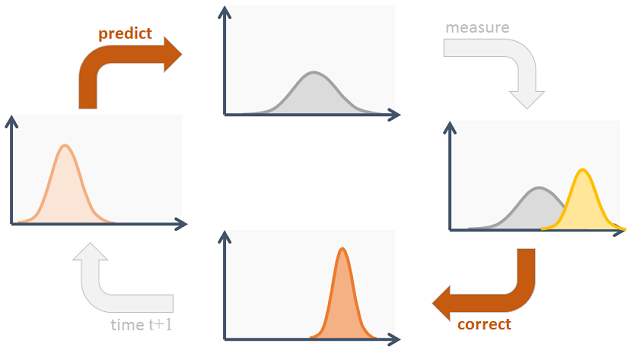
\includegraphics[scale=0.4]{report/pic/2/kf_workflow.jpeg} 
  \caption{A heuristic viw of Kalman Filter workflow.}
\end{figure}
\subsubsection{Kalman filter}
Kalman filtering [12] provides a way of using observation and prediction of data comprehensively, considering the effect of system and environment noise. State estimation based on Kalman filter will be more accurate than relying solely on observation, as it cannot be fully precise.\\
In the circumstance of tracking, players’ locations are what we need to track, and historical information recorded for a player is saved in a tracklet maintained for him/her in temporal sequence. For each player, his/her location for current frame is first predicted based on historical information using the filter. The prediction is based on assumption that player moves almost linearly between fames, so formula for predicting can then be elicited:\\
\begin{align*}
x_k = x_{k-1}+v_{k-1}^x \\
y_k = y_{k-1}+v_{k-1}^y
\end{align*}
where 
\begin{align*}
v_{k-1}^a = a_{k-1} - a_{k-2}, \: a=x \: \text{or} \:y
\end{align*}
\\
After corresponding detection is found, it is then combined with the prediction made to give the final location of the player in current frame. Again, a prediction for next frame is made. This is done for every frame to keep position of players updated, their historical information saved in tracklets, hence tracking is achieved.
\subsubsection{Temporal coherence}
The method of determining which detection should be assigned to which tracklet is not simply assigning a detection to a tracklet in which previous detections have the same label as classification result is likely to be erroneous, instead, it is based on temporal coherence. People cannot run too fast, thus the distance they move between frames must be under a certain limit.\\
Base on this common sense, we can set a hyperparameter defining the maximal distance a player can move in each frame. After matching potential pairs of tracklets and new detections, we check if Euclidean distance between each pair of prediction made through Kalman filter and detection is smaller than this threshold. Qualified distance leads to a detection combining with paired prediction to give final location of corresponding player, otherwise the detection will be rejected by tracklet as they are potential errors.
\newpage
\section{Development}
In this section, all method I tried for system implementation are described.
\subsection{System workflow}
Before the system starts to work, models for player detection and player classification are prepared. A target broadcast video will be gone through twice. In the first iteration, for each frame, detections are found, their labels are given by classification model, and assigned to tracklets. After this iteration finished, tracklets that only consists of false positives are filtered out and label correction is done on each remained tracklet. They are then sorted according to temporal sequence of the first frame. At last, tracklets are drawn on target video in the second iteration.\\
\subsection{Player detection}
\subsubsection{Heuristics}
Some heuristics are used to eliminate false positives to some degree and speed up detection.\\
One pre knowledge is that in a footage from static camera, the area representing pitch remain unchanged throughout frames.
Also, players cannot run out of pitch. Consequently, for every frame a sub image that only contains pitch and players with in is cropped out for detection. This can accelerate detection process, since less areas need to be swept through, and reduce false positives, as any of them that will appear out of pitch region in the original region will no longer appear in the cropped one.\\
\begin{figure}
  \centering
  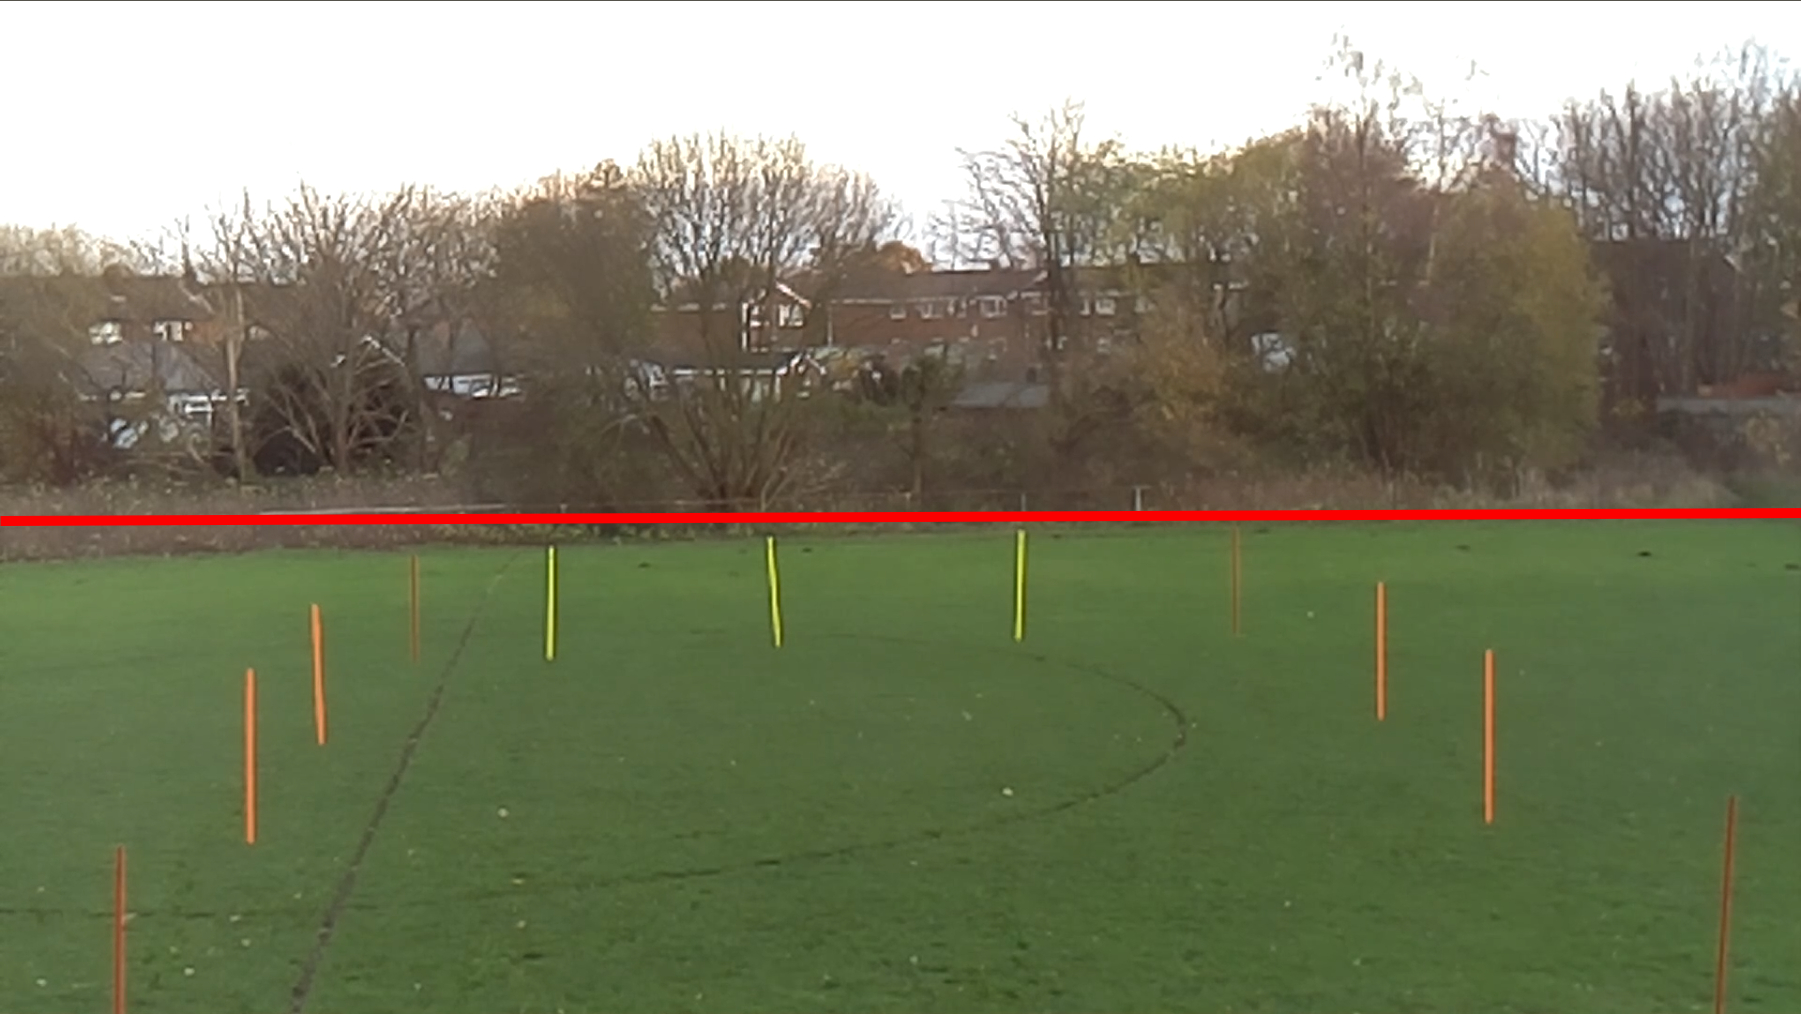
\includegraphics[scale=0.2]{report/pic/3/background.jpg} 
  \caption{Pure background, only region under red line will be used in detection.}
\end{figure}
\begin{figure}
  \centering
  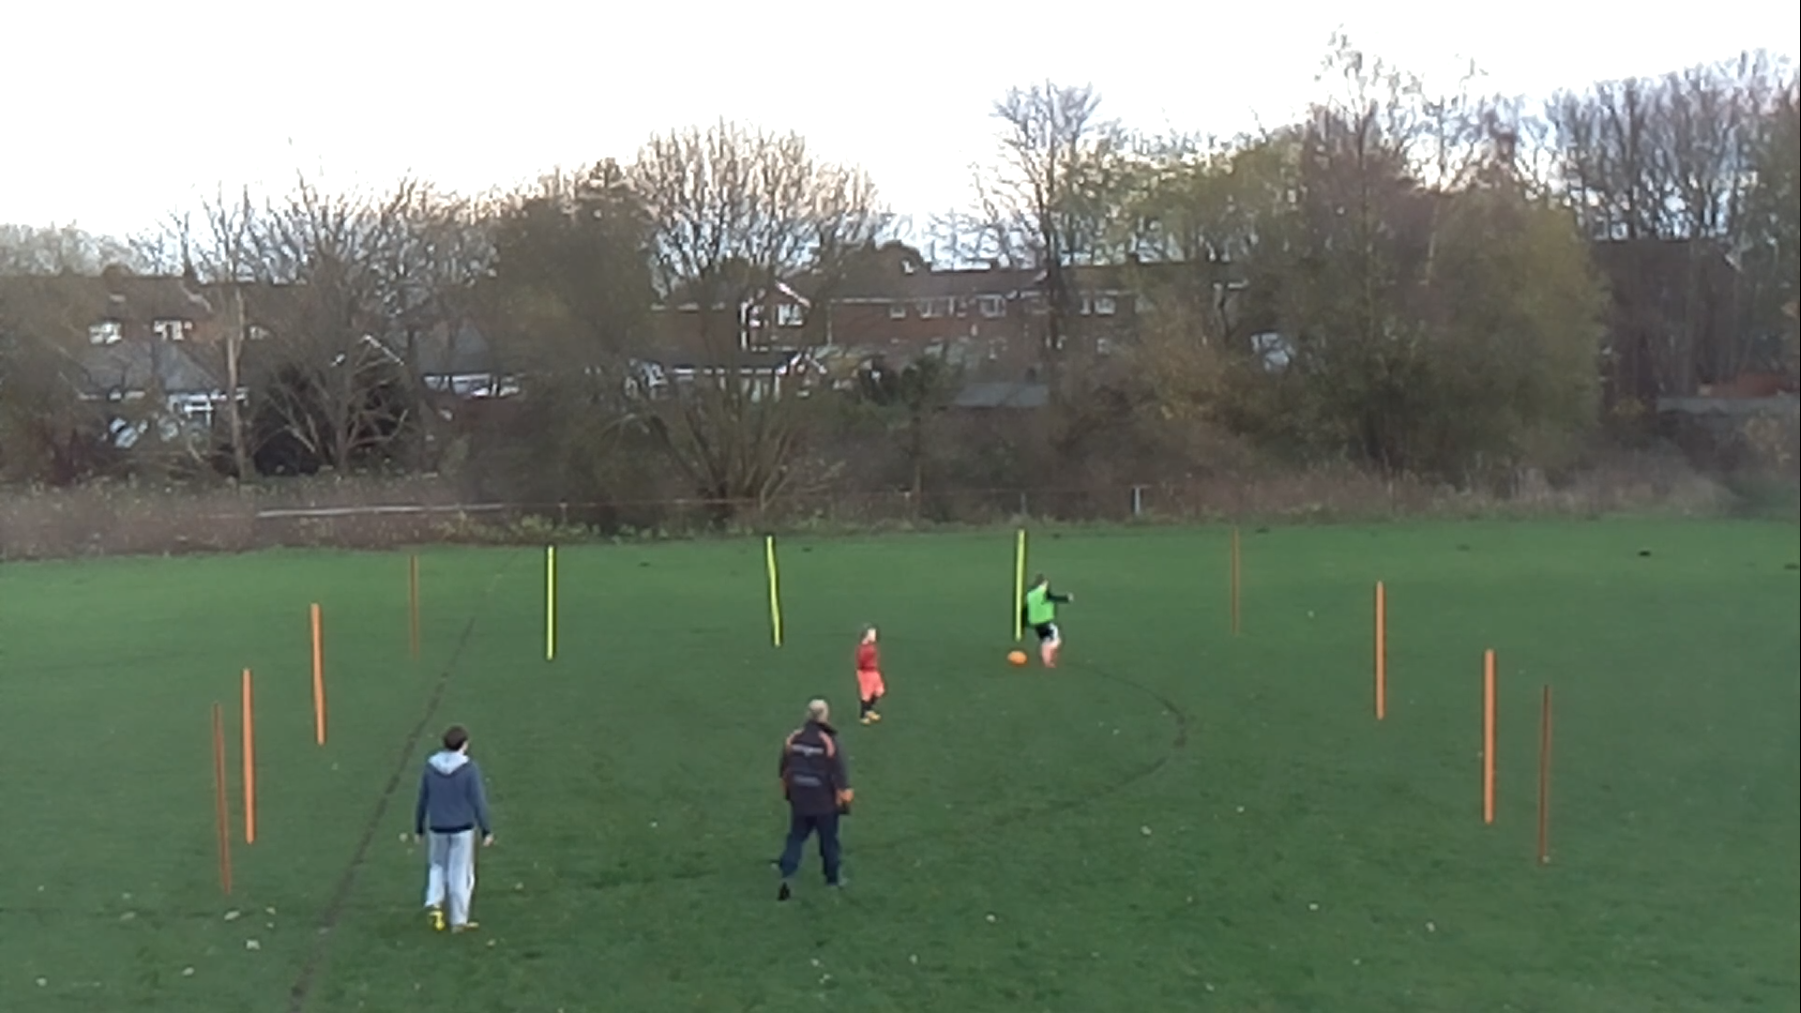
\includegraphics[scale=0.2]{report/pic/3/foreground.png} 
  \caption{Background with players.}
\end{figure}
Secondly, bounding box of a player should be neither too large nor too small, neither too slim nor too wide. Although scale of players may vary as they ran towards or away from camera, it should still between a certain range. So, boxes that do not have its size fall in the range should also be discarded.
\subsubsection{Background subtraction}
At first, I tried to use background subtraction for detection baseline. For a static video its background remains unchanged, thus making it plausible to capture a pure background frame and subtract it from every other frame to get foreground information.\\
The background subtraction algorithm implementation I used is from OpenCV [13], it is achieved base on Gaussian Mixture Model (GMM).  \\
As we can see from Figure 9 \& 10, in the dataset the foreground (players \& football) is easily distinguishable from background, thus we can expect their pixel values are clearly different. Heuristically, for each frame I get, we can simply do the subtraction and blobs we get marks location of player.\\
At first, background model will be subtracted from the frame and updated with background pixels. The difference image then goes through a threshold to filter out shadows captured.\\
The blobs too small represents background and noise points, so here a threshold is applied to filter them out. For rest of the blobs, findcontours [14] from OpenCV is used to draw a bounding box around each of them by using maximum and minimum information of x, y coordinates kept in obtained contour. It has an advantage that the rectangle is drawn stick with blob, thus marking precisely the player’s location and include little extra information.\\
Some detection result examples are shown below.\\
\begin{figure}[h!]
  \begin{subfigure}[b]{\linewidth}
  \centering
    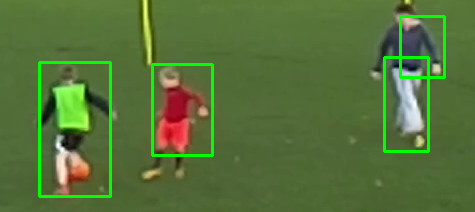
\includegraphics[scale=0.4]{report/pic/3/multi_box_2.png} 
  \end{subfigure}
  \begin{subfigure}[b]{\linewidth}
  \centering
    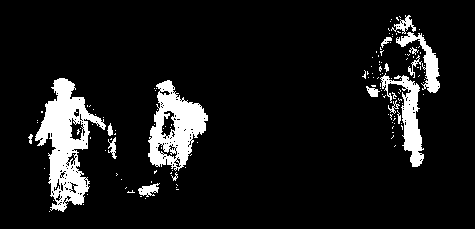
\includegraphics[scale=0.4]{report/pic/3/multi_box_1.png} 
  \end{subfigure}
  \caption{Sometimes bounding boxes cannot cover the whole player due to incomplete blob.}
\end{figure}
\begin{figure}[h!]
  \centering
  \begin{subfigure}[b]{0.4\linewidth}
    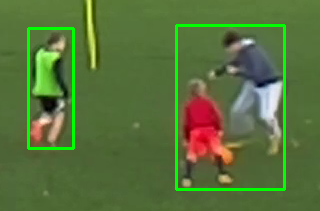
\includegraphics[scale=0.4]{report/pic/3/occlusion_1.png} 
  \end{subfigure}
  \begin{subfigure}[b]{0.4\linewidth}
    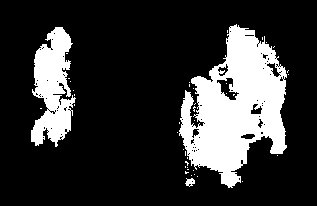
\includegraphics[scale=0.4]{report/pic/3/occlusion_0.png} 
  \end{subfigure}
  \caption{Background subtraction not being able to subtract players.}
\end{figure}
From the examples above we can see that background subtraction have some shortcomings that may seriously hinder later steps.\\
First, it is too vulnerable to occlusion. When occlusion occurs, in the subtracted image we can only know there are something different from background, but we don’t know it represents 2 people as there are only one blob. Other information that may help us judge that here are two people are lot after subtraction process.\\
Second, blob for a player may not be always connected, causing the bounding box cannot cover the whole player.\\
I made an attempt to at least solve the third problem by adding several iterations of dilation then several iterations of erosion to connect blobs belong to the same person in order to give exactly 1 bounding box for 1 player with the correct size.\\
\begin{figure}[h!]
  \begin{subfigure}[b]{\linewidth}
  \centering
    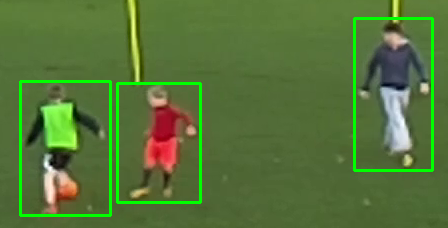
\includegraphics[scale=0.4]{report/pic/3/complete_blob_1.png} 
  \end{subfigure}
  \begin{subfigure}[b]{\linewidth}
  \centering
    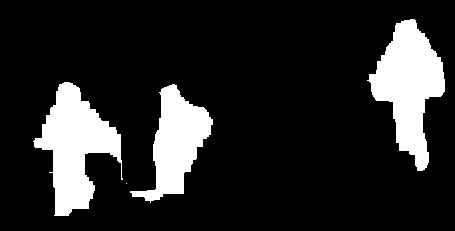
\includegraphics[scale=0.4]{report/pic/3/complete_blob.png} 
  \end{subfigure}
  \caption{Using dilation to fill blob \& erosion to restore blob size.}
\end{figure}
We can see that some how the third problem is solved, yet other 2 problems are still difficult to deal with using background subtraction.
\subsubsection{SVM detector based on HOG}
Then I migrate to use an SVM detector. An SVM detector should first be prepared. For each frame, a sliding window will sweep across the whole frame, and each window is then put into the classifier to see if it contains a person. I tried to used a pretrained classifier in OpenCV [15] and a self-trained one.
\paragraph{Pretrained classifier}
This classifier is trained on INRIA dataset, thus being a general purpose one. Given the common sense that boundaries of human beings are similar and HOG feature mainly describe edges, I propose a guess that sports players may also have similar HOG features with non-sportsperson. Thus, a general-purpose detector may have acceptable result on sportsperson detection.\\
\begin{figure}[h!]
  \centering
  \begin{subfigure}[b]{0.4\linewidth}
    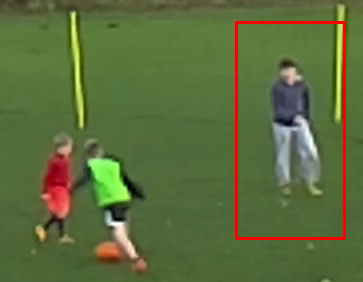
\includegraphics[scale=0.4]{report/pic/3/vulnerability_to_occlusion_1.png} 
  \end{subfigure}\hspace{5mm}
  \begin{subfigure}[b]{0.4\linewidth}
    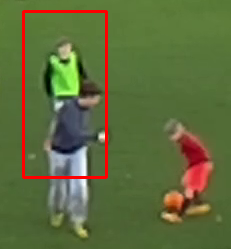
\includegraphics[scale=0.5]{report/pic/3/vulnerbility_to_occlusion_2.png} 
  \end{subfigure}
  \caption{Failure to occlusion.}
\end{figure}
The results above actually denied my guess. We can see that the general-purpose detector gives too many false negatives, thus cannot provide enough detections to do continuous tracking. The reason may be that the dataset INRIA itself is not general enough – it only contains examples of pedestrians, yet HOG features of pedestrians are mutually similar but obviously different from those of sports players who often has more varied pose.
\paragraph{Self-trained classifier}
Then I decided to train a linear SVM detector based on HOG features using the given football dataset. OpenCV has implementation of HOG feature computation [16] and SVM classifier [17], so I only need to provide training data here. \\
After training examples are loaded, a 64*128 sub image of each example is first cropped to fit sliding window size defined in the SVM implementation. Then HOG features are computed and put into the classifier for training. After the training completes, hard negative mining is used and obtained fale negatives are again put into the classifier for further training to improve its accuracy.\\
Using the self-trained classifier for detection should be in the same way as we use the pre-trained one, only this time load the self-trained SVM classifier.\\
At first, I did not realize to apply heuristics of scanning only the region below the redline in Figure9 and only used given datasete to train my SVM. The result proved to be rather noisy:
\begin{figure}[h!]
  \begin{subfigure}[b]{\linewidth}
  \centering
    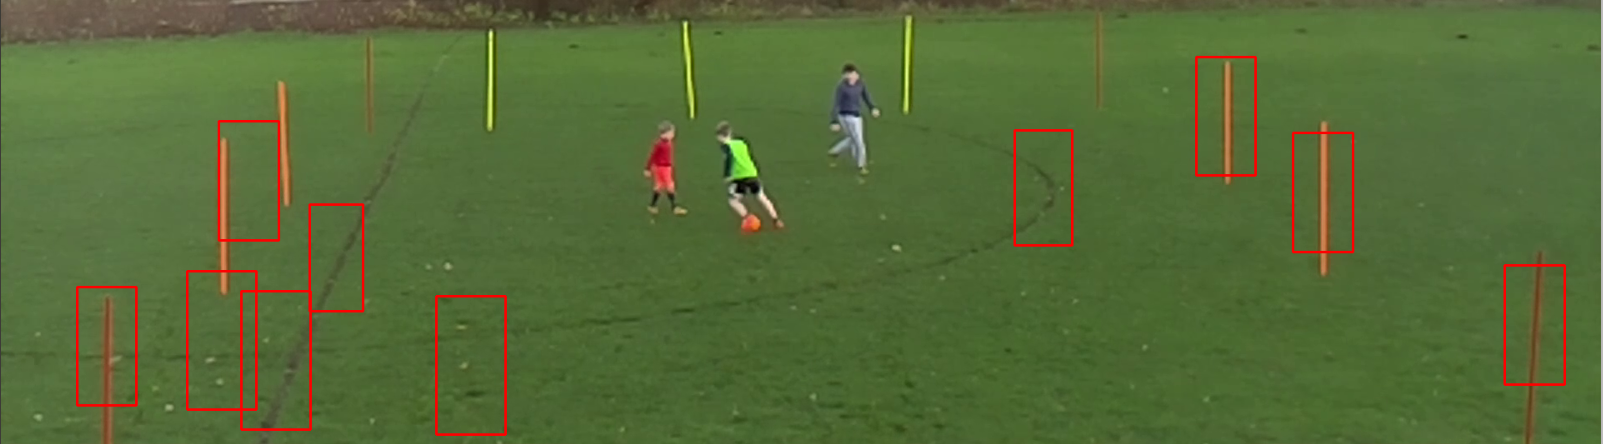
\includegraphics[scale=0.2]{report/pic/3/selfHOG_1stround_2.png} 
  \end{subfigure}
  \begin{subfigure}[b]{\linewidth}
  \centering
    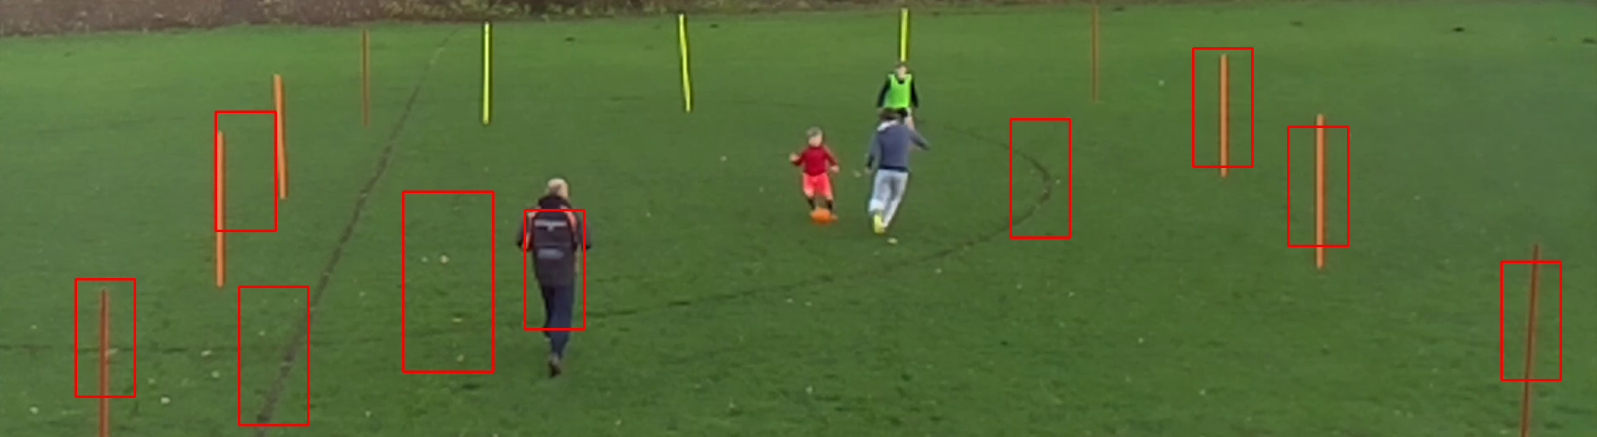
\includegraphics[scale=0.2]{report/pic/3/selfHOG_1stround_1.png} 
  \end{subfigure}
  \caption{Too many fasle positive but almost no true positive.}
\end{figure}

\begin{figure}[h!]
  \begin{subfigure}[b]{\linewidth}
  \centering
    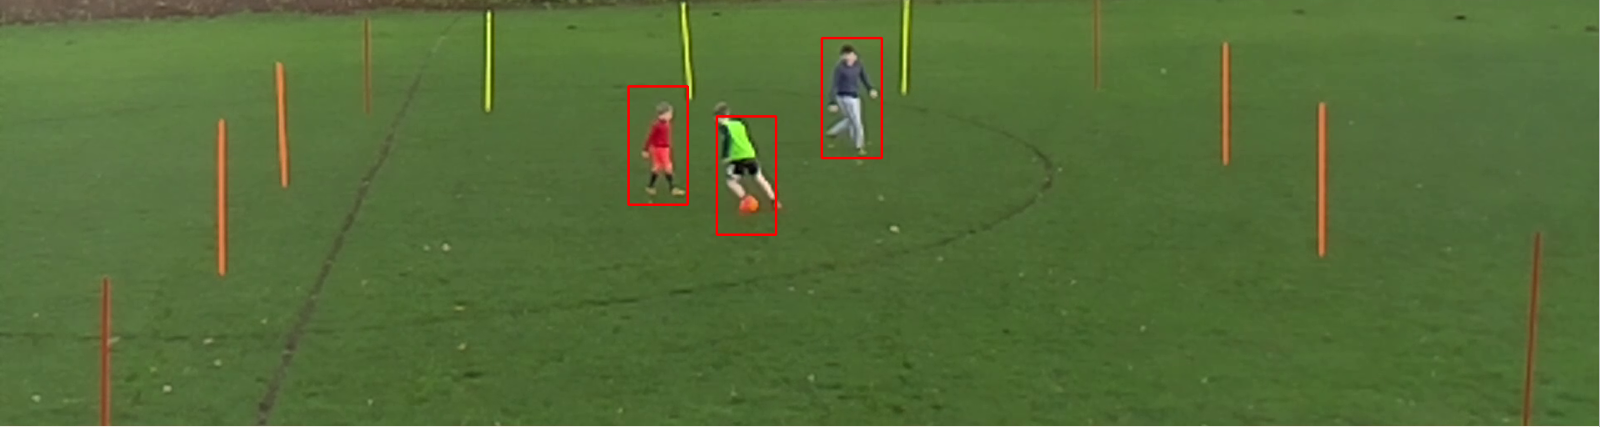
\includegraphics[scale=0.2]{report/pic/3/selfHOG_2ndround_1.png} 
  \end{subfigure}
  \begin{subfigure}[b]{\linewidth}
  \centering
    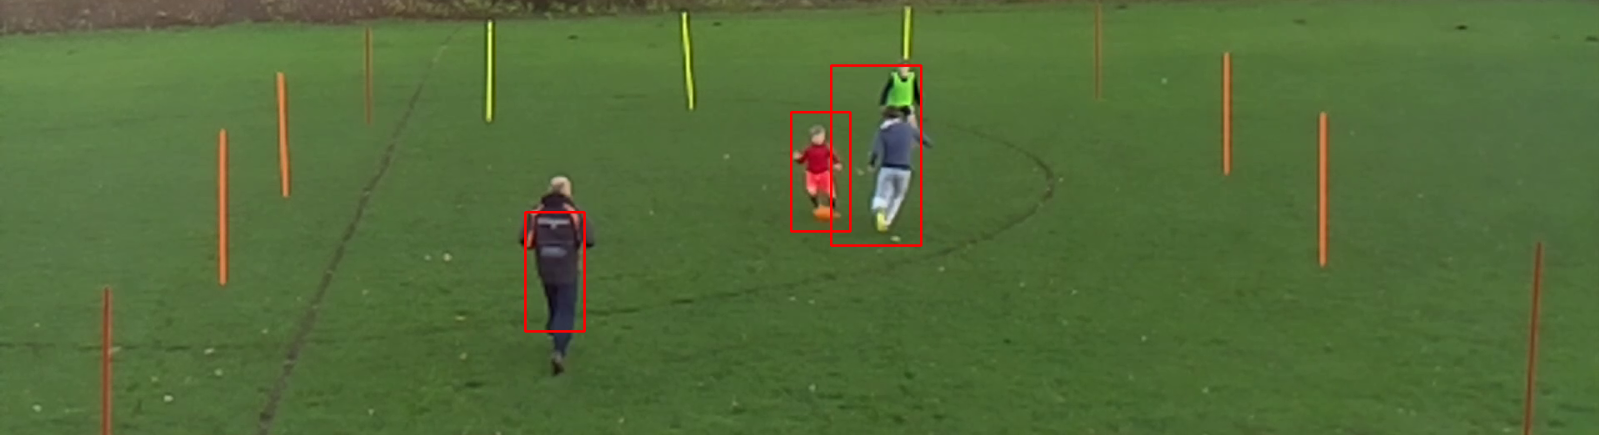
\includegraphics[scale=0.2]{report/pic/3/selfHOG_2ndround_2.png} 
  \end{subfigure}
  \begin{subfigure}[b]{\linewidth}
  \centering
    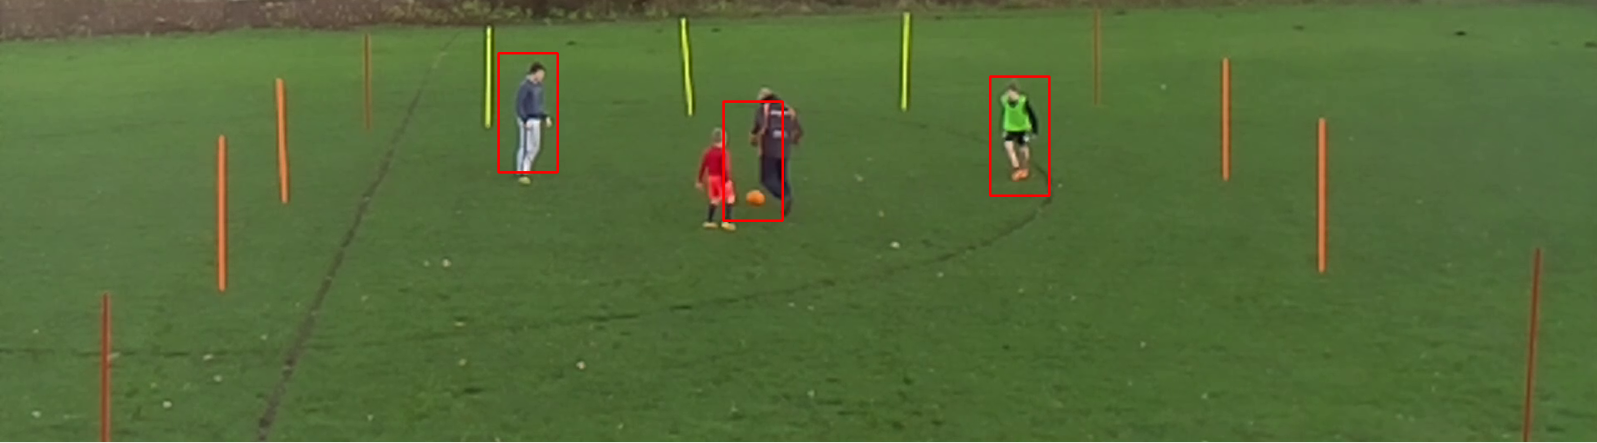
\includegraphics[scale=0.2]{report/pic/3/selfHOG_2ndround_3.png} 
  \end{subfigure}
  \begin{subfigure}[b]{\linewidth}
  \centering
    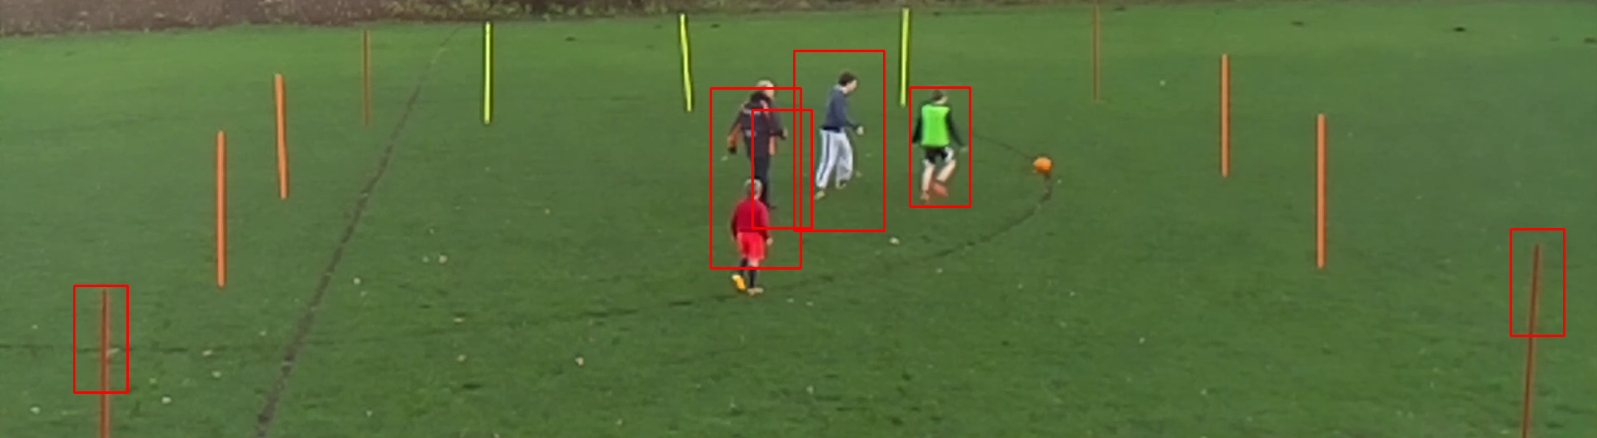
\includegraphics[scale=0.2]{report/pic/3/selfHOG_2ndround_4.png} 
  \end{subfigure}
  \caption{False positive almost eliminated, but still vulnerable at occlusion.}
\end{figure}

\begin{figure}[h!]
  \begin{subfigure}[b]{\linewidth}
  \centering
    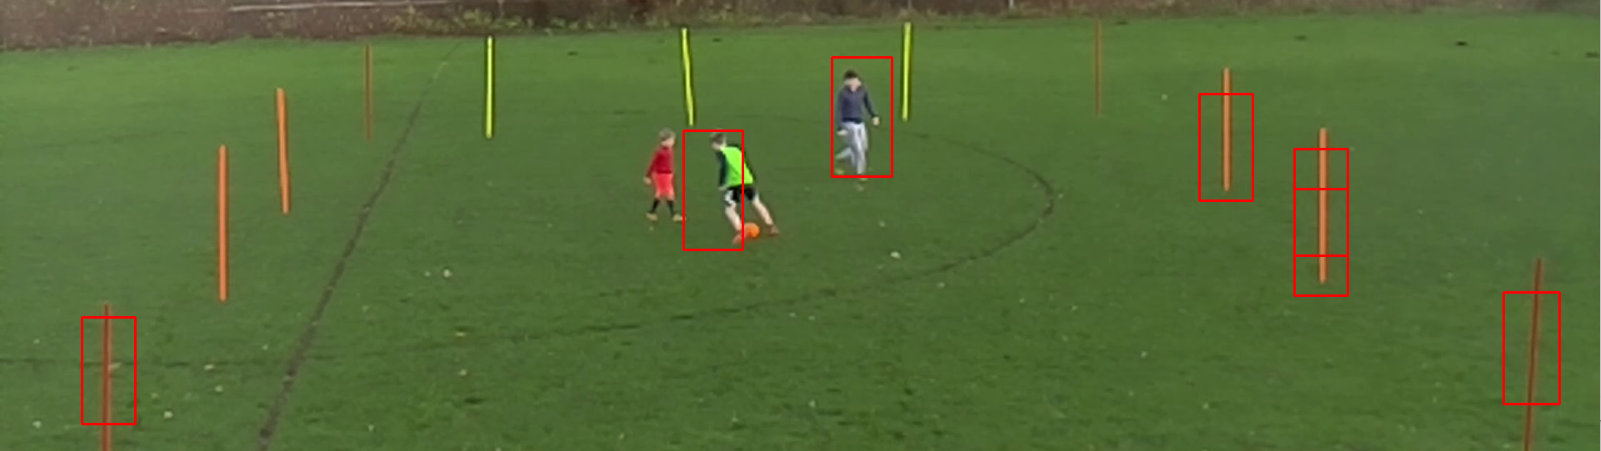
\includegraphics[scale=0.2]{report/pic/3/selfHOG_3rdround_1.png} 
  \end{subfigure}
  \begin{subfigure}[b]{\linewidth}
  \centering
    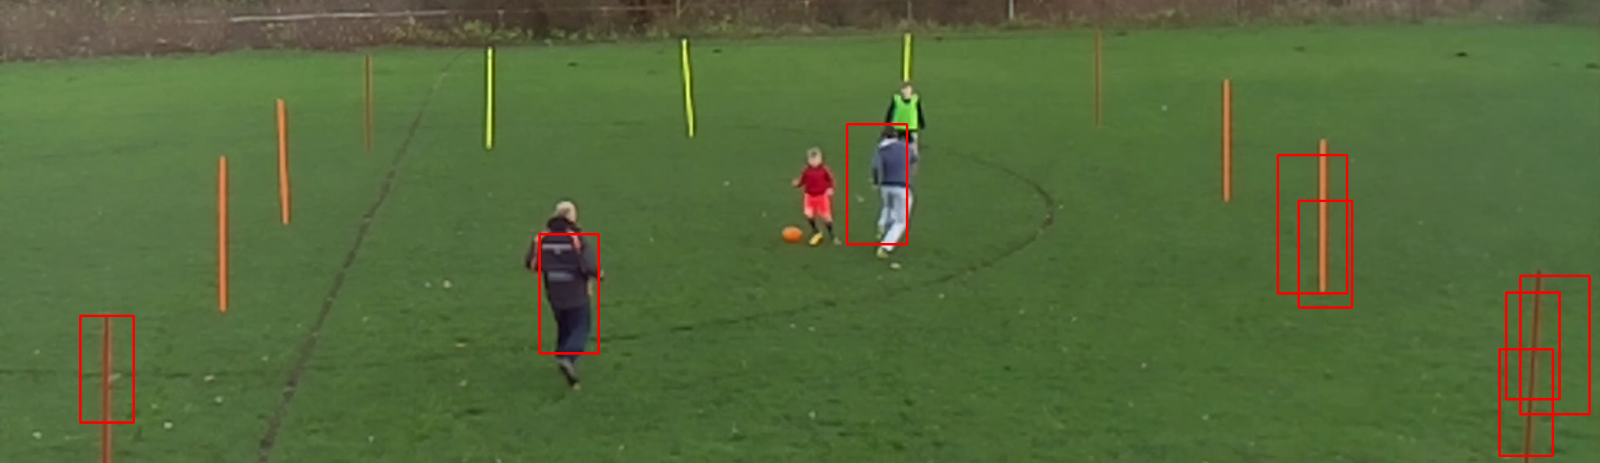
\includegraphics[scale=0.2]{report/pic/3/selfHOG_3rdround_2.png} 
  \end{subfigure}
  \begin{subfigure}[b]{\linewidth}
  \centering
    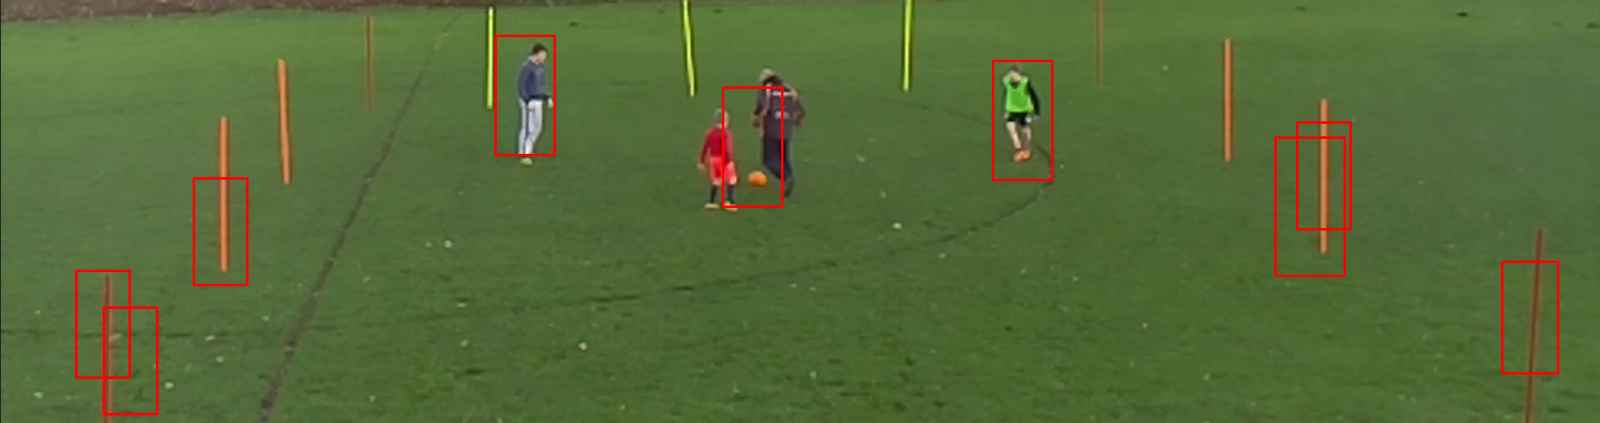
\includegraphics[scale=0.2]{report/pic/3/selfHOG_3rdround_3.png} 
  \end{subfigure}
  \begin{subfigure}[b]{\linewidth}
  \centering
    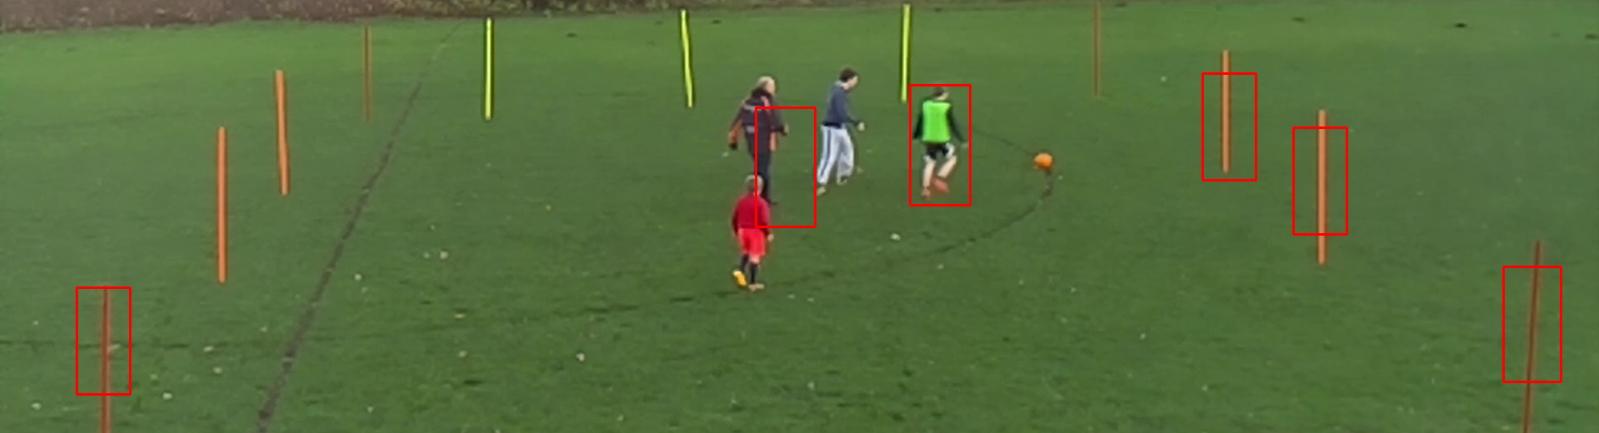
\includegraphics[scale=0.2]{report/pic/3/selfHOG_3rdround_4.png} 
  \end{subfigure}
  \caption{False positives appear again, while occluson problem not migitated.}
\end{figure}

\begin{figure}[h!]
  \begin{subfigure}[b]{\linewidth}
  \centering
    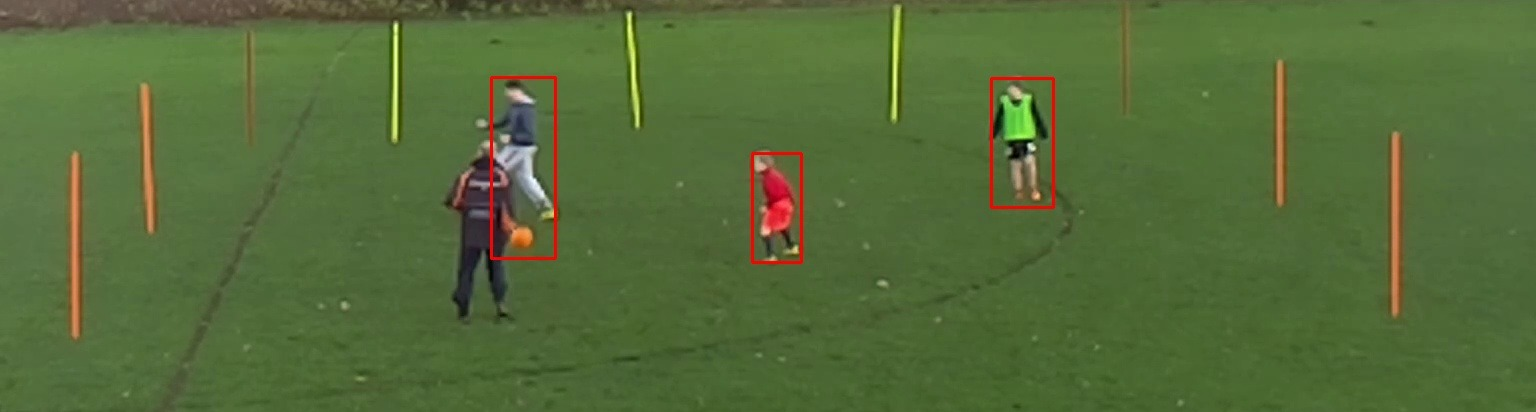
\includegraphics[scale=0.2]{report/pic/3_new/det_occlu.jpg}
    \caption{Detection success when slight occlusion occurs.}
  \end{subfigure}
  \begin{subfigure}[b]{\linewidth}
  \centering
    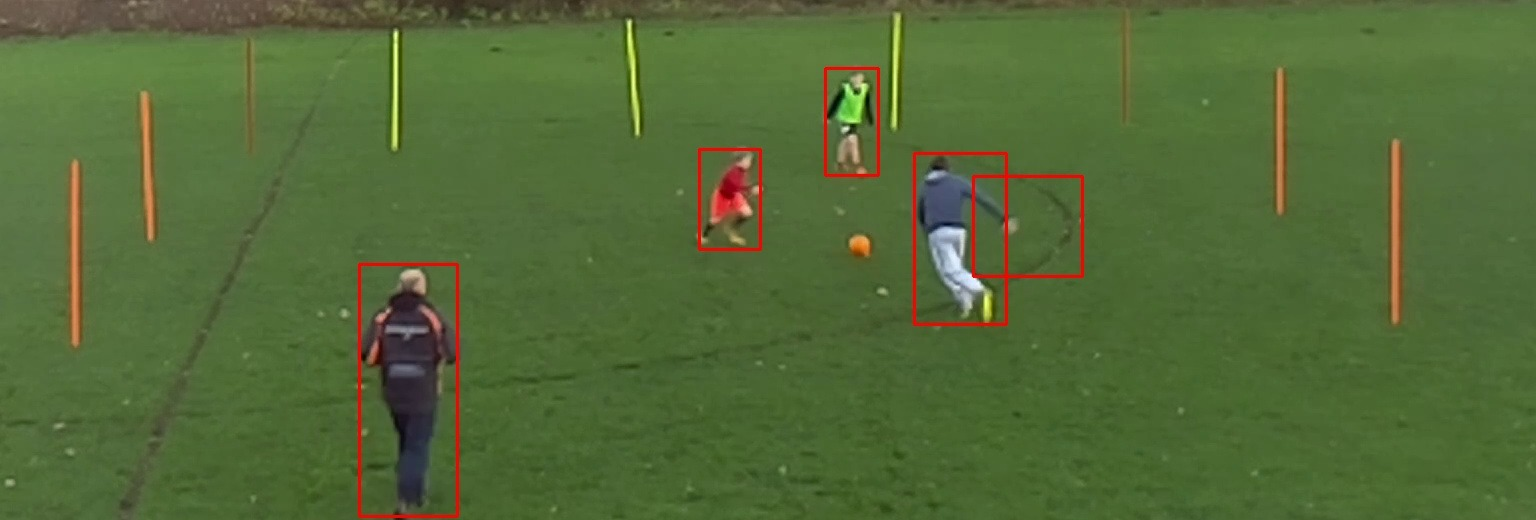
\includegraphics[scale=0.2]{report/pic/3_new/false_posi.jpg} 
    \caption{False positives detected.}
  \end{subfigure}
  \begin{subfigure}[b]{\linewidth}
  \centering
    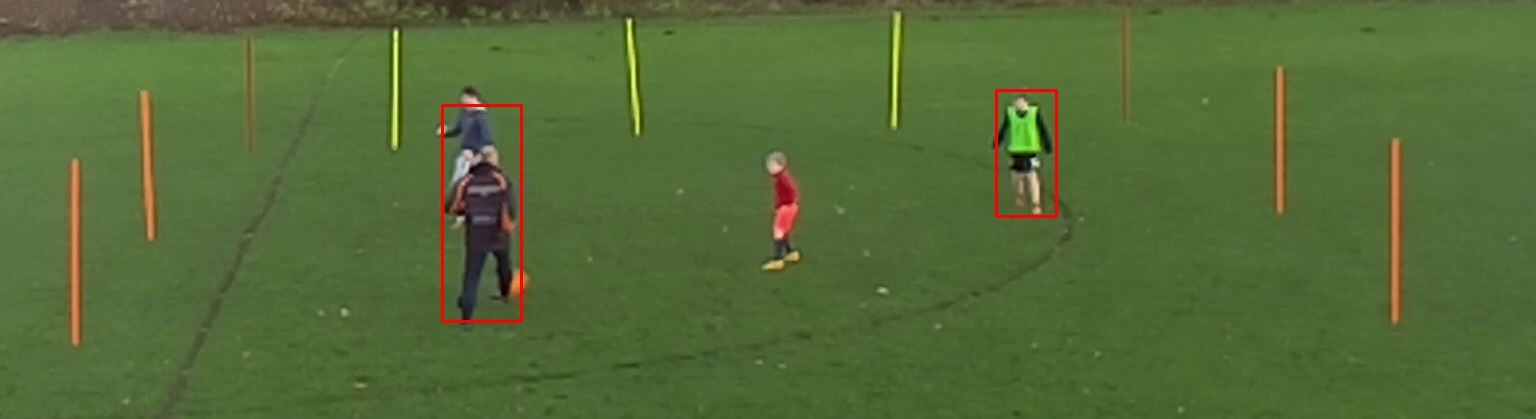
\includegraphics[scale=0.2]{report/pic/3_new/failure.jpg} 
    \caption{Detection failure at severe occlusion and at other players.}
  \end{subfigure}
  \caption{Mask-RCNN detection result example.}
\end{figure}

(Figure 15)There are too many false positives and number of true positives is too low, so I output detections and pick more positive and negative examples to further train the classifier. I did this several times until false positives almost don’t appear.\\
(Figure 16)We can see that this time the classifier can give more continuous detection , yet another problem still exists: It is vulnerable to occlusion in a different way: the detector fails to detect players that are near each other. I guess there may be too few true positives describing occlusion, so I further added examples of occlusion into training examples.\\
However, (Figure 17)false negatives began to appear again before problem at occlusion is solved. Since training SVM on too large dataset is rather time consuming, continue adding false negatives will not be a good idea.
My guess is that after those examples are added, the SVM hyperparameter can no longer put all positive examples at one side and there are more negative examples at the positive side. This shall be a problem of hyperplane lacking non-linearity.
\subsubsection{Detector from Mask-RCNN network}
Speaking of adding non-linearity, a neural network is especially good at doing that. What’s more, compared to SVM’s limitation on types of kernel tricks, a neural network can achieve far more complex hyperplanes. The Mask-RCNN network implementation I used is from [18] and there are minor adjusting to the code to fit a newer version of Keras framework.\\
The model is trained on MS COCO dataset [18], it contains photos of 91 types of objects, including human,thus the model is also a general-purpose one. Instead of using only one type of feature, more comprehensive ones are extracted due to how convolution layers work.\\
Player detection work is like testing phase for a neural network. A frame is fed into the Mask-RCNN and output will be instance segmentation result for it, including a colored mask,a label and a bounding box for every recognized object. Here we only use bounding boxes produced.
\paragraph{Heuristic at occlusion}
No matter how powerful the model is against occlusion, it still fails when occlusion is too severe. To somehow mitigate this, an extra heuristic is proposed.\\
Normally, the bounding box of a player cannot change suddenly in size when moving to the next frame. However, when occlusion starts to hinder detection result, bounding box of one player will disappear and that of the other will suddenly get larger. 
So when such a circumstance occurs, and distance between the box that grow larger than a certain threshold and the one disappears is close enough, we know occlusion takes place, and the large, single box will be dismantled into two smaller ones according to its actual location and prediction of where the 2 smaller boxes should have been.\\
There are two ways that a box may be dismantled, as shown in Figure 19:\\
If 2 players are coming close to each other from top-left and bottom-right(judgement is made based on locationdata of players in the frevious frame, when occlusion did not occur yet), then the box will be dismantled into one at top-left and the other at bottom-right with their sizes are the same as ones in previous frames; if they are coming from top-right and bottom-left, then the new boxes will be createdon the top-left and bottom-right corner.

\begin{figure}[h!]
  \begin{subfigure}[b]{\linewidth}
  \centering
    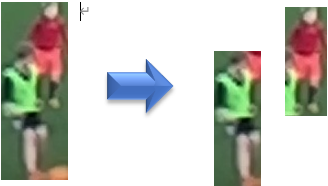
\includegraphics[scale=0.5]{report/pic/3/heuristic_1.PNG} 
    \caption{Splitting top-left and bottom-right.}
  \end{subfigure}
  \begin{subfigure}[b]{\linewidth}
  \centering
    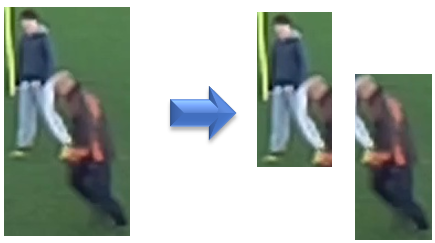
\includegraphics[scale=0.5]{report/pic/3/heuristic_2.PNG} 
    \caption{Splitting top-right and bottom-left.}
  \end{subfigure}
  \caption{}
\end{figure}

\begin{figure}[h!]
  \begin{subfigure}[b]{0.5\linewidth}
  \centering
	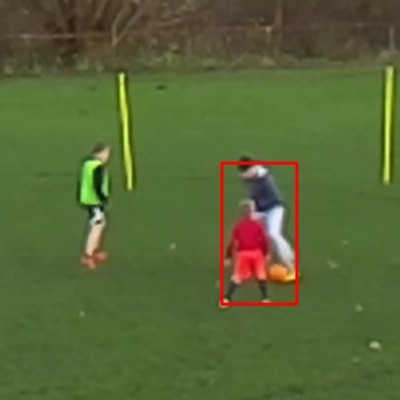
\includegraphics[scale=0.4]{report/pic/3_new/off_1.jpg} 
  \end{subfigure}
  \begin{subfigure}[b]{0.5\linewidth}
  \centering
	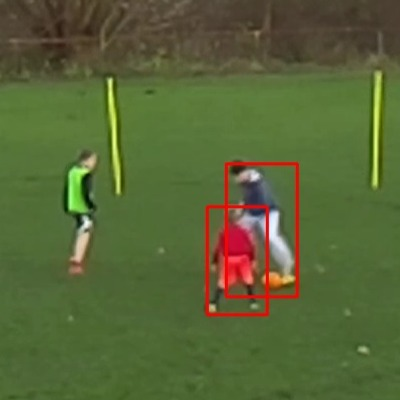
\includegraphics[scale=0.4]{report/pic/3_new/on_1.jpg} 
  \end{subfigure}
  \begin{subfigure}[b]{0.5\linewidth}
  \centering
	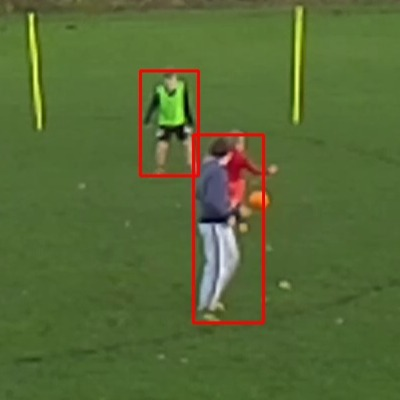
\includegraphics[scale=0.4]{report/pic/3_new/off_2.jpg} 
  \end{subfigure}
  \begin{subfigure}[b]{0.5\linewidth}
  \centering
	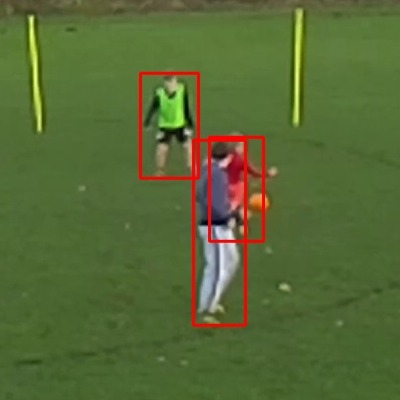
\includegraphics[scale=0.4]{report/pic/3_new/on_2.jpg} 
  \end{subfigure}
  \begin{subfigure}[b]{0.5\linewidth}
  \centering
	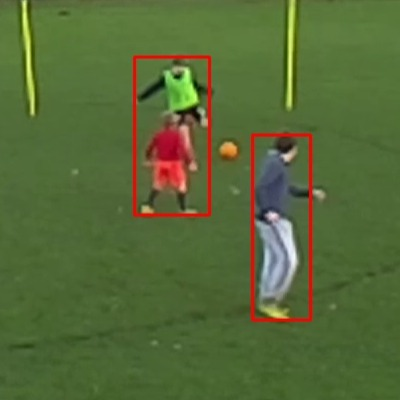
\includegraphics[scale=0.4]{report/pic/3_new/off_3.jpg} 
  \end{subfigure}
  \begin{subfigure}[b]{0.5\linewidth}
  \centering
	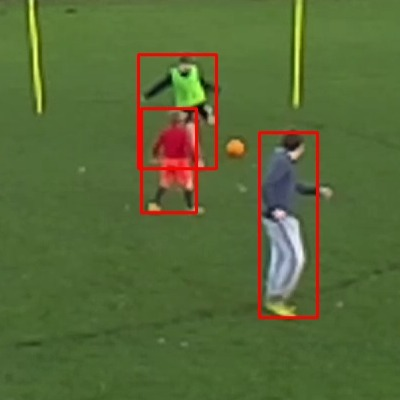
\includegraphics[scale=0.4]{report/pic/3_new/on_3.jpg} 
  \end{subfigure}
  \caption{Detection result comparison. Left: heuristic off; Right: heuristic on.}
\end{figure}

\begin{figure}[h!]
  \begin{subfigure}[b]{0.5\linewidth}
  \centering
	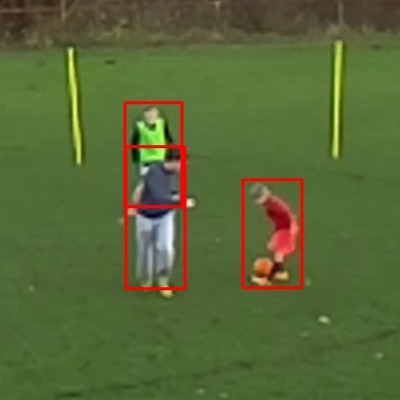
\includegraphics[scale=0.4]{report/pic/3_new/off_seq_1.jpg} 
  \end{subfigure}
  \begin{subfigure}[b]{0.5\linewidth}
  \centering
	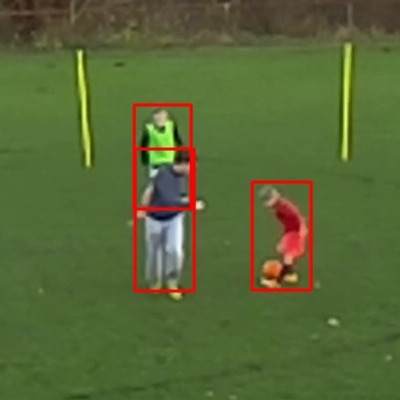
\includegraphics[scale=0.4]{report/pic/3_new/on_seq_1.jpg} 
  \end{subfigure}
    \begin{subfigure}[b]{0.5\linewidth}
  \centering
	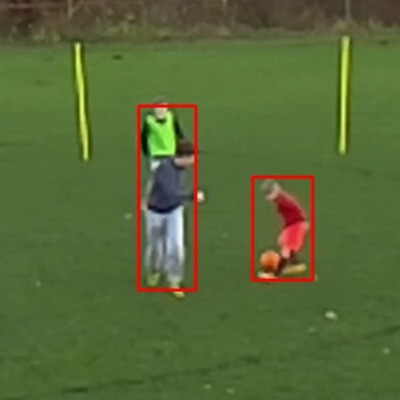
\includegraphics[scale=0.4]{report/pic/3_new/off_seq_2.jpg} 
  \end{subfigure}
  \begin{subfigure}[b]{0.5\linewidth}
  \centering
	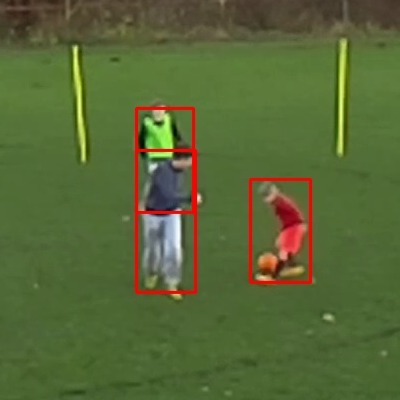
\includegraphics[scale=0.4]{report/pic/3_new/on_seq_2.jpg} 
  \end{subfigure}
    \begin{subfigure}[b]{0.5\linewidth}
  \centering
	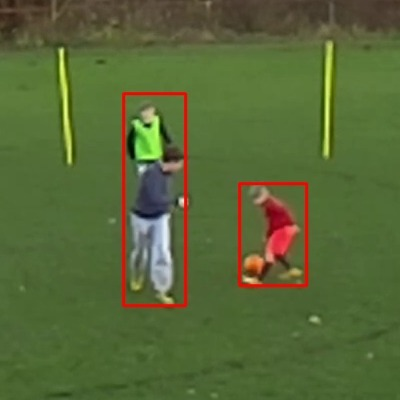
\includegraphics[scale=0.4]{report/pic/3_new/off_seq_3.jpg} 
  \end{subfigure}
  \begin{subfigure}[b]{0.5\linewidth}
  \centering
	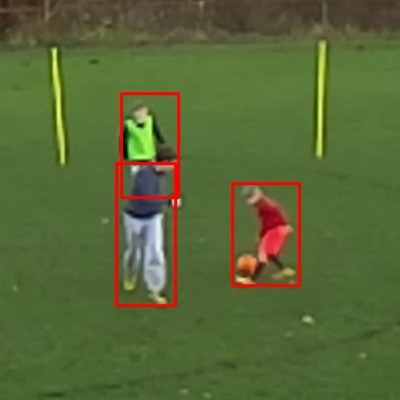
\includegraphics[scale=0.4]{report/pic/3_new/on_seq_3.jpg} 
  \end{subfigure}
  \caption{A detection sequence result comparison(part 1). Left: heuristic off; Right: heuristic on.}
\end{figure}

\begin{figure}[h!]
  \begin{subfigure}[b]{0.5\linewidth}
  \centering
	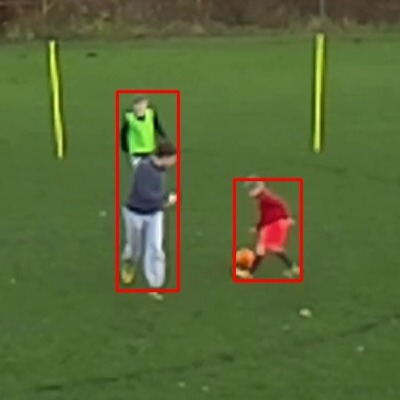
\includegraphics[scale=0.4]{report/pic/3_new/off_seq_4.jpg} 
  \end{subfigure}
  \begin{subfigure}[b]{0.5\linewidth}
  \centering
	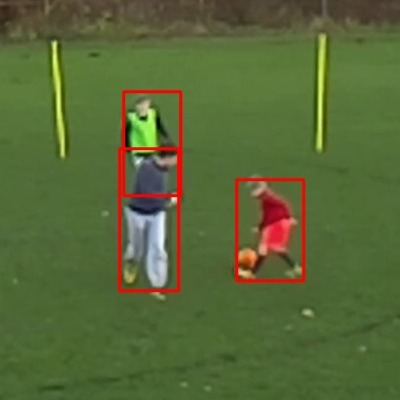
\includegraphics[scale=0.4]{report/pic/3_new/on_seq_4.jpg} 
  \end{subfigure}
    \begin{subfigure}[b]{0.5\linewidth}
  \centering
	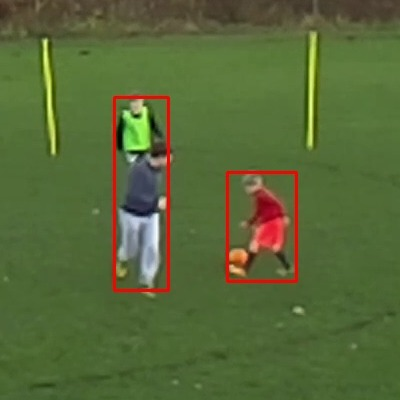
\includegraphics[scale=0.4]{report/pic/3_new/off_seq_5.jpg} 
  \end{subfigure}
  \begin{subfigure}[b]{0.5\linewidth}
  \centering
	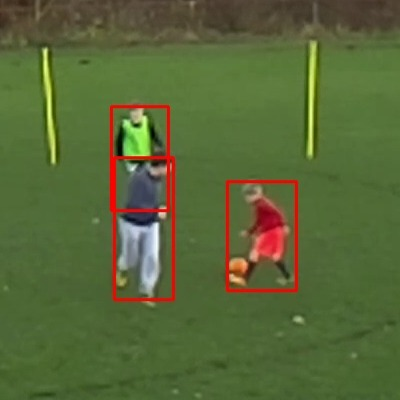
\includegraphics[scale=0.4]{report/pic/3_new/on_seq_5.jpg} 
  \end{subfigure}
    \begin{subfigure}[b]{0.5\linewidth}
  \centering
	\includegraphics[scale=0.4]{report/pic/3_new/off_seq_6.jpg} 
  \end{subfigure}
  \begin{subfigure}[b]{0.5\linewidth}
  \centering
	\includegraphics[scale=0.4]{report/pic/3_new/on_seq_6.jpg} 
  \end{subfigure}
  \caption{A detection sequence result comparison(part 2). Left: heuristic off; Right: heuristic on.}
\end{figure}

\begin{figure}[h!]
  \begin{subfigure}[b]{0.5\linewidth}
  \centering
	\includegraphics[scale=0.4]{report/pic/3_new/heu_false_off.jpg} 
  \end{subfigure}
  \begin{subfigure}[b]{0.5\linewidth}
  \centering
	\includegraphics[scale=0.4]{report/pic/3_new/heu_false_on.jpg} 
  \end{subfigure}
  \caption{False positive given by heuristic. Left: heuristic off; Right: heuristic on.}
\end{figure}

\subsection{Player identification}
After players are detected in each frame, I then need to use a calssifier to give each player an identification. This identification is not directly used in the next part--tracking, instead it act as ground truth data at final label correction level.\\
Taking into consideration that the examples are of low resolution and assigning identification in sport footage is a very task-specific problem, the classifier needs to be self-trained on example data.\\ 
The classification model I utilized is from [1]. At first, I also tried to use hyperparameters recommended in its evaluation part, where only SIFT featuer is used, k=11 and size of bag of words is 200, yet this did not perform well in my system so further experiment is done, and finally my configuration is using SIFT based on MSERs, k=11 and size of bag of words is 75.
\subsection{Tracking}
The approach of tracking-by-detection is applied in this partm meaning that trakcing is based on detection instead of identification. A tracklet is created to store a sequence of detections of a player, however, there is likely to be more number of tracklets produced from a footage than number of players appeared in it, because a player will enter and exit the scene several times, and a player may be lost track due to occlusion. If number of tracklets is hard-coded as the same as maximum number of players in footage, then it is likely that In some tracklets there will be large intervals of useless data due to player abscent from the scene, storing all these information of absense will lead to huge waste of memory space. Therefor is may not be a good idea to hard-code numer of tracklets.\\
The way I implement the tracking step is based on [2], with Kalman filter used for correction and prediction.
A problem mentioned in [2] is that when occlusion occurs a tracklet may sometimes lose track of the corresponding player, this is because in the context of football, occlusion often happens when an attacker tries to bypass the defender and this alway involves complex moving techniques that will cause change to original moving direction. The tracking point will also move irreguarly in frames before we actual detection of the player disappears due to sharp change of shape of bounding box, causing extra disruption to prediction. Consequently when prediction goes in one way, the player actually goes in another direction and the problem of losing track occurs.\\
To somehow migitate the problem, a slightly more complex prediction model is used. When an actual detection is matched for the tracklet, everything will work as [2]. When actual detection disappears and we can only rely on prediction, a variable $c$ is used.\\
$c$ records currently how many mere predictions are used to store player location since the last actual detection appears. When an actual detection is matched with current tracklet, $c$ is always 0; when it is the first frame that only prediction is used, $c$=1; when it is the second frame, $c$=2, etc.\\
$e^{-c}$ is used to gradually slow down the speed of predicted detection inthe hope that it may not leave actual detection so far, so the final transition matrix used in Kalman filter is actually:\\
\[\begin{bmatrix}1 & e^{-c}\frac{x_{k-1}-x_{k-2}}{y_{k-1}} \\e^{-c}\frac{y_{k-1}-y_{k-2}}{x_{k-1}} & 1 \end{bmatrix}\].\\
Note that when actuall detection is matched, c=0, so $e^{-c}$=1, and the matrix becomes the one used in [2].\\
\subsection{Tracklet cleaning \& Label Correction}
Here more works are done to filter out obviously erronous tracklets and give a consistent label across the tracklet.
\subsubsection{Tracklet cleaning}
In the stage of detection, most of false positives contain more than one players(which happens at occlusion), yet there are still a few false positives that contains no players. In mose cases they appear in one frame then disappears instantly, and may appear again at least hundreds of frames later. According to the scheme of tracking, this kind of false positives are likely to have new tracklets constructed on them as they will be filtered out by temporal coherence of every tracklet(since continuous detection can be almost achieved when occlusion did not occur, all tracklets will be first matched with a detection of player). Such tracklets will only contain 1 actual detection so their tracklet will be obviously shorter than those of players. So simply applying a threshold on length of tracklet shall convenitntly filter them out.
\subsubsection{Label correction}
Here the baseline method is implemented.
After a running through of target broadcast video, Tracklets will contain full trajectory information of a player, however, since detections in a tracklet may still be different due to the way we assign detections in tracking step. Here a majority label voting is done on each tracklet to give its final label.
Here the majority vote is only done on actual detections. In my implementation, all label of predicted detections will use that of the last actual detection before the player is lost track, however, the label of the last actual detection may be wrong as player classification is far from perfect, meaning that all labels of predicted locations may be wrong. Consequently they cannot be used for determining final label of the tracklet.
\begin{figure}[h!]
  \begin{subfigure}[b]{\linewidth}
  \centering
    \includegraphics[scale=0.2]{report/pic/3_new/no_occlusion.png} 
    \caption{Success at normal case.}
  \end{subfigure}
  \begin{subfigure}[b]{\linewidth}
  \centering
    \includegraphics[scale=0.2]{report/pic/3_new/success.png} 
    \caption{Success when occlusion occurs.}
  \end{subfigure}
  \begin{subfigure}[b]{\linewidth}
  \centering
    \includegraphics[scale=0.2]{report/pic/3_new/false_identity.png} 
    \caption{A player given false identity.}
  \end{subfigure}
  \begin{subfigure}[b]{\linewidth}
  \centering
    \includegraphics[scale=0.2]{report/pic/3_new/false_negative.png} 
    \caption{Tracking failure.}
  \end{subfigure}
  \caption{Tracking failure.}
  \begin{subfigure}[b]{\linewidth}
  \centering
    \includegraphics[scale=0.2]{report/pic/3_new/occlu_fail.png} 
    \caption{Failure at occlusion.}
  \end{subfigure}
  \caption{Example results of final system.}
\end{figure}

\subsection{Display}
Then we can draw results on target footage. There are 3 things drawn for each player:
\begin{itemize}
\item 1. A bounding box marking location, with its color specific for each player;
\item 2. Player identification result given above the bounding box, it also determines color used to print the text and draw bounding box.
\item 3. A curve marks current trajectory of the player with its color the same as bounding box.
\end{itemize}
Product video is output as a \texttt{.mp4} file for review. Tracklet that stores identification and trajectory are also produced as a intermediate result but also can be further make use of.
\subsection{Test}
Although techniques I tried are similar to those in [1] and [2], yet the first part of the system-player detection has a different final method deployed, and hyperparameter configuration I get for player classification is also diferent, so the evaluation of the whole ystem should aso be done from scratch. These works are recorded in the next section.
\newpage

\section{Evaluation}
\subsection{Detection}
\subsubsection{Data collection}
Some preprocessing is done on training and testing videos to shorten data collection time. For trainingVideo.mp4, data collection starts at 00:24 where the 2nd player enters the camera frame, for testingVideo.mp4 it starts at 00:22, where the first 2 players appeared; and ends at 4:43, when no more occlusion occurs in the video.
Ground truth data is needed to do evaluation here. The method I used is basically the same as that in [1], except for the bounding boxes are got using model from Mask-RCNN network.
\subsubsection{Evaluation standard}
Ideally, a successful detection should include (approximately) the whole body of a player; in practice, detection of player entering the frame should also be considered; in the meanwhile, detections that only contains some body parts of a player or multiple players should be considered false positives.\\
Quality of detection is evaluated after basic heuristics are applied to filter out those obvious false detections, or to say, only evaluated on detections that are to be classified and put into tracklets later, as these are detections that will affect how the system perform as a whole. Detections filtered out at the beginning do not have influence on performance of the system.\\
Unlike the method of setting number of players(note as $\#$oP) as a parameter of evaluation program in [1] to estimate total number of detections in a video, I calculate total number of player occurrences in a more fine-grained way:\\
Taking into consideration that players will enter and exit the camera frame from time to time, I first estimate frame intervals in which $\#$oP is of a certain value. This can be nearly accurate by stopping at whenever number of players change and record the index of current frame. Between each of 2 continuous records $\#$oP remain unchanged. By multiplying $\#$oP and length of the interval and adding it up on all intervals, total number of $\#$oP occurrences in a footage can be given more accurately than simply multiplying most common $\#$oP with video length.\\
Detections in a footage are gathered automatically, and manual justification is done to distinguish true positives from false ones, as This justification of whether a detection is o the whole body of a player(sometimes including occluded parts) cannot be easily done. \\
\subsubsection{Evaluation \& experiments}
In the text below, player A represents the person in blue, player B is the one in green jersey, player C is the one in red, Scott is the one in black.\\
Manual review is done on detections to distinguish false positives from true ones. Tneir numbers are counted and preciion and recall given.\\
True positive: detections that contain the whole body of only one player. It is acceptable that some parts are occluded or the bounding box also contains body parts of other players.\\
\begin{figure}[h!]
\centering
  \begin{subfigure}[b]{0.15\linewidth}
  \centering
    \includegraphics[scale=0.4]{report/pic/4/pos_1.jpg} 
    \caption{}
  \end{subfigure}
  \begin{subfigure}[b]{0.15\linewidth}
  \centering
    \includegraphics[scale=0.4]{report/pic/4/pos_2.jpg} 
    \caption{}
  \end{subfigure}
  \begin{subfigure}[b]{0.15\linewidth}
  \centering
    \includegraphics[scale=0.4]{report/pic/4/pos_3.jpg}
    \caption{} 
  \end{subfigure}
  \caption{example of true positives.}
\end{figure}

\begin{figure}[h!]
\centering
  \begin{subfigure}[b]{0.25\linewidth}
  \centering
    \includegraphics[scale=0.4]{report/pic/4/neg_1.jpg} 
    \caption{}
  \end{subfigure}
  \begin{subfigure}[b]{0.25\linewidth}
  \centering
    \includegraphics[scale=0.4]{report/pic/4/neg_2.jpg} 
    \caption{}
  \end{subfigure}
  \begin{subfigure}[b]{0.25\linewidth}
  \centering
    \includegraphics[scale=0.4]{report/pic/4/neg_3.jpg}
    \caption{} 
  \end{subfigure}
  \begin{subfigure}[b]{0.25\linewidth}
  \centering
    \includegraphics[scale=0.4]{report/pic/4/neg_4.jpg} 
    \caption{}
  \end{subfigure}
  \begin{subfigure}[b]{0.25\linewidth}
  \centering
    \includegraphics[scale=0.4]{report/pic/4/neg_5.jpg} 
    \caption{}
  \end{subfigure}
  \begin{subfigure}[b]{0.25\linewidth}
  \centering
    \includegraphics[scale=0.4]{report/pic/4/neg_6.jpg} 
    \caption{}
  \end{subfigure}
  \caption{example of false positives.}
\end{figure}
False positive: detections that contains full body parts of more than one players, background object or only background without players. \\
Figure 19 shows some example of true positives.
\begin{itemize}
\item (a): Bounding box containing exactly a player.
\item (b): Bounding box containing a player partially occluded by another, yet the lower boundary is likely to stick to the feet of Scott.
\item (c): Bounding box containing multiple players, but the edge of the box stick to the boundary of player A.
\end{itemize}
When a box only includes parts of a player due to he/she is entering or leaving the scene, it is seen as a true positive.\\
Figure 20 shows some example of false positives.
\begin{itemize}
\item (a): Bounding box containing a player and othr stuff.
\item (b),(c): Bounding box containing multiple players. 
\item (d): Blank too wide above or below a player.
\item (e): Bounding box with no player.
\item (f): Bounding box contain only body parts of multiple players.
\end{itemize}
When a box only includes parts of a player due to occlusion, it is seen as a false positive.\\
In the two videos I tested on, We can roughly know the time that a player enters or leaves the scene(it is not frequent), so it is easy to judge due to what reason a partial inclusion in the bounding box of a player happened.
According to the way I count number of player occurences above, there are 28795 occurences in shortened testingVideo.mp4/4peopleKickabout 25fps.mp4 and 36319 occurences in shortened trainingVideo.m4/4peopleKickabout2 30fps.mp4.\\
By manually going through the detection results of the 2 videos, I discovered that detections of player C is fewer of other players. This happens due to 2 reasons:
\begin{itemize}
\item a. Occlusion occurs frequently. Player C appears smaller in size in the scene, and due to low resolution, it is particularly hard to do image segmentation to propose a possible bounding box in Region Proposal Network, especally when player C goes behind another one(sometimes the player will be completely occluded).
\item b. Heuristic threshold on bounding box size is used to filter out those only contain parts of a player. However, when player C goes too far from camera, its bounding box size will also gets below the threshold, being another dilemma on whether to improve precision or recall. My choice here is to increase precision.
From these experiment results, we can see that the detector has a rather high recall with relatively lower precision, meaning that it is powerful at making detections correct: Almost all detections it gives contain the whole body of exactly one player. However, it is relatively weaker on detecting players. Detection failure happens almost entirely due to partial and full occlusion, as it can be observed from video that detections are almost continuous when players are not occluded.
\end{itemize}
From Table 1-5 we can see that the heuristic on splitting bounding box when occlusion occurs do help increase both precision and recall. Generally, lower splitting threshold value set will lead to higher precision and recall. Since performance of the detector shall be the same when no occlusion occuss, we may likely to conlcude that such a heuristic do help migitating problem of occlusion.\\
However, this is still a very primitive model and only works on an occlusion of 2 players. When the change is caused by 3 or more players coming close and occlude each other ath the same time, in only rare cases will the heuristic still give proper splitting result as their possible trajectory combinations becomes much more complex.\\
\begin{table}[]
\centering
\begin{tabular}{|c|c|c|c|c|c|}
\hline
\multicolumn{3}{|c|}{trainingVideo} & \multicolumn{3}{c|}{testingVideo} \\ \hline
 & True & False &  & True & False \\ \hline
Positive & 24046 & 1140 & Positive & 19721 & 1121 \\ \hline
Negative &  & 12273 & Negative &  & 8179 \\ \hline
precision & \multicolumn{2}{c|}{93.25\%} & precision & \multicolumn{2}{c|}{94.62\%} \\ \hline
recall & \multicolumn{2}{c|}{63.21\%} & recall & \multicolumn{2}{c|}{68.49\%} \\ \hline
\end{tabular}
\caption{Confusion matrix with no heuristic applied}
\end{table}

\begin{table}[]
\centering
\begin{tabular}{|c|c|c|c|c|c|}
\hline
\multicolumn{3}{|c|}{trainingVideo} & \multicolumn{3}{c|}{testingVideo} \\ \hline
 & True & False &  & True & False \\ \hline
Positive & 25042 & 848 & Positive & 20583 & 794 \\ \hline
Negative &  & 11277 & Negative &  & 8212 \\ \hline
precision & \multicolumn{2}{c|}{96.72\%} & precision & \multicolumn{2}{c|}{96.29\%} \\ \hline
recall & \multicolumn{2}{c|}{68.95\%} & recall & \multicolumn{2}{c|}{73.01\%} \\ \hline
\end{tabular}
\caption{Confusion matrix when th=1.2}
\end{table}

\begin{table}[]
\centering
\begin{tabular}{|c|c|c|c|c|c|}
\hline
\multicolumn{3}{|c|}{trainingVideo} & \multicolumn{3}{c|}{testingVideo} \\ \hline
 & True & False &  & True & False \\ \hline
Positive & 24823 & 990 & Positive & 20402 & 927 \\ \hline
Negative &  & 11496 & Negative &  & 8393 \\ \hline
precision & \multicolumn{2}{c|}{96.16\%} & precision & \multicolumn{2}{c|}{95.65\%} \\ \hline
recall & \multicolumn{2}{c|}{68.34\%} & recall & \multicolumn{2}{c|}{72.36\%} \\ \hline
\end{tabular}
\caption{Confusion matrix when th=1.25}
\end{table}

\begin{table}[]
\centering
\begin{tabular}{|c|c|c|c|c|c|}
\hline
\multicolumn{3}{|c|}{trainingVideo} & \multicolumn{3}{c|}{testingVideo} \\ \hline
 & True & False &  & True & False \\ \hline
Positive & 24987 & 778 & Positive & 20421 & 956 \\ \hline
Negative &  & 11332 & Negative &  & 7663 \\ \hline
precision & \multicolumn{2}{c|}{96.98\%} & precision & \multicolumn{2}{c|}{95.53\%} \\ \hline
recall & \multicolumn{2}{c|}{68.80\%} & recall & \multicolumn{2}{c|}{70.92\%} \\ \hline
\end{tabular}
\caption{Confusion matrix when th=1.3}
\end{table}

\begin{table}[]
\centering
\begin{tabular}{|c|c|c|c|c|c|}
\hline
\multicolumn{3}{|c|}{trainingVideo} & \multicolumn{3}{c|}{testingVideo} \\ \hline
 & True & False &  & True & False \\ \hline
Positive & 24805 & 933 & Positive & 20303 & 956 \\ \hline
Negative &  & 11514 & Negative &  & 8492 \\ \hline
precision & \multicolumn{2}{c|}{96.37\%} & precision & \multicolumn{2}{c|}{95.50\%} \\ \hline
recall & \multicolumn{2}{c|}{68.30\%} & recall & \multicolumn{2}{c|}{70,50\%} \\ \hline
\end{tabular}
\caption{Confusion matrix when th=1.35}
\end{table}
\subsection{Classification}
My evaluation on result of player identification roughly follows the idea used in [1], where different combinations of parameters are tested, hyperparameters adjusted and confusion matrix given. However, a more detailed result is presented for convenience of analysis.\\
Sometimes precision and recall of each class vary lagely. As our final goal is to maximize precision and recall of all classes, only giving average value may be inappropriate as particularly low valus cannot be noticed in this case. Consequently, precision and recall of each class is given, and overall accuracy is also listed as a reference.
\begin{table}[]
\centering
\begin{tabular}{|c|c|c|c|c|c|c|c|c|c|}
\hline
\multicolumn{1}{|l|}{by \%} & \multicolumn{4}{l|}{precision} & \multicolumn{4}{l|}{recall} & \multirow{2}{*}{Accuracy} \\ \cline{1-9}
\multicolumn{1}{|l|}{bin size} & A & B & C & scott & A & B & C & scott &  \\ \hline
16 & 89.47 & 9.30 & 34.18 & 87.90 & 1.96 & 2.54 & 99.69 & 69.34 & 43.38 \\ \hline
32 & 84.91 & 24.06 & 41.99 & 91.39 & 5.84 & 19.76 & 94.53 & 78.46 & 49.65 \\ \hline
64 & 72.13 & 22.58 & 42.33 & 91.40 & 8.46 & 22.38 & 87.92 & 74.46 & 48.31 \\ \hline
\end{tabular}
\caption{RGB histogrm with K=11}
\end{table}

\begin{table}[]
\begin{tabular}{|c|c|c|c|c|c|c|c|c|c|}
\hline
\multicolumn{1}{|l|}{by \%} & \multicolumn{4}{c|}{precision} & \multicolumn{4}{c|}{recall} & \multicolumn{1}{l|}{\multirow{2}{*}{accuracy}} \\ \cline{1-9}
BOW size & A & B & C & scott & A & B & C & scott & \multicolumn{1}{l|}{} \\ \hline
25 & 88.53 & 94.41 & 90.01 & 94.54 & 89.07 & 87.25 & 92.92 & 98.07 & 91.83 \\ \hline
50 & 94.69 & 93.97 & 89.56 & 96.23 & 89.92 & 91.83 & 94.07 & 98.42 & 93.56 \\ \hline
75 & 95.68 & 95.35 & 92.04 & 96.15 & 92.15 & 92.53 & 95.26 & 99.15 & 94.77 \\ \hline
100 & 94.47 & 94.87 & 93.25 & 96.05 & 92.11 & 94.11 & 94.11 & 98.34 & 94.67 \\ \hline
125 & 95.85 & 94.94 & 94.31 & 95.17 & 92.53 & 94.07 & 95.11 & 98.53 & 95.05 \\ \hline
150 & 96.79 & 94.69 & 93.93 & 95.13 & 91.73 & 94.88 & 95.38 & 98.46 & 95.11 \\ \hline
200 & 97.04 & 95.67 & 95.55 & 93.23 & 92.27 & 94.61 & 95.84 & 98.57 & 95.32 \\ \hline
\end{tabular}
\caption{MSER with K=11}
\end{table}

\begin{table}[]
\begin{tabular}{|c|c|c|c|c|c|c|c|c|c|}
\hline
\multicolumn{1}{|l|}{by \%} & \multicolumn{4}{c|}{precision} & \multicolumn{4}{c|}{recall} & \multicolumn{1}{l|}{\multirow{2}{*}{accuracy}} \\ \cline{1-9}
BOW size & A & B & C & scott & A & B & C & scott & \multicolumn{1}{l|}{} \\ \hline
25 & 77.24 & 74.65 & 71.22 & 92.46 & 64.5 & 62.42 & 95.30 & 91.61 & 78.46 \\ \hline
50 & 76.68 & 87.16 & 67.79 & 97.11 & 73.61 & 55.61 & 98.69 & 91.88 & 79.95 \\ \hline
63 & 80.75 & 87.95 & 63.75 & 97.36 & 69.38 & 56.19 & 98.96 & 92.46 & 79.25 \\ \hline
75 & 80.49 & 91.01 & 61.95 & 97.61 & 71.88 & 51.80 & 99.23 & 91.38 & 78.57 \\ \hline
87 & 84.34 & 93.08 & 59.25 & 98.87 & 70.65 & 52.30 & 99.34 & 91.31 & 78.41 \\ \hline
100 & 86.21 & 96.04 & 56.73 & 98.95 & 69.5 & 50.46 & 99.42 & 90.65 & 77.50 \\ \hline
125 & 85.78 & 95.44 & 52.04 & 99.36 & 61.03 & 45.15 & 99.5 & 89.76 & 73.86 \\ \hline
\end{tabular}
\caption{SIFT with K=11}
\end{table}

\begin{table}[]
\begin{tabular}{|c|c|c|c|c|c|c|c|c|c|}
\hline
\multicolumn{1}{|l|}{by \%} & \multicolumn{4}{c|}{precision} & \multicolumn{4}{c|}{recall} & \multicolumn{1}{l|}{\multirow{2}{*}{accuracy}} \\ \cline{1-9}
BOW size & A & B & C & scott & A & B & C & scott & \multicolumn{1}{l|}{} \\ \hline
25 & 91.60 & 84.59 & 86.90 & 96.89 & 82.30 & 84.5 & 96.5 & 96.15 & 89.86 \\ \hline
50 & 91.62 & 91.37 & 83.82 & 97.76 & 85.42 & 81.53 & 98.84 & 97.38 & 90.79 \\ \hline
75 & 90.30 & 94.27 & 83.76 & 98.96 & 87.80 & 79.11 & 99.19 & 99.38 & 91.37 \\ \hline
100 & 94.85 & 98.09 & 84.74 & 99.19 & 90.69 & 85.19 & 99.38 & 99.46 & 93.68 \\ \hline
150 & 96.41 & 98.46 & 80.32 & 99.38 & 85.76 & 86.19 & 99.53 & 98.96 & 92.61 \\ \hline
150 & 97.95 & 99.22 & 78.18 & 99.26 & 86.38 & 84.07 & 99.53 & 99.03 & 92.25 \\ \hline
\end{tabular}
\caption{SIFT+MSER with K=11}
\end{table}

\begin{table}[]
\begin{tabular}{|c|c|c|c|c|c|c|c|c|c|}
\hline
\multicolumn{1}{|l|}{by \%} & \multicolumn{4}{c|}{precision} & \multicolumn{4}{c|}{recall} & \multicolumn{1}{l|}{\multirow{2}{*}{accuracy}} \\ \cline{1-9}
\begin{tabular}[c]{@{}c@{}}Feature \\ combined\end{tabular} & A & B & C & scott & A & B & C & scott & \multicolumn{1}{l|}{} \\ \hline
SIFT & 72.13 & 22.59 & 42.34 & 91.40 & 8.46 & 22.38 & 87.96 & 74.46 & 48.31 \\ \hline
MSER & 72.13 & 22.59 & 42.34 & 91.40 & 8.46 & 22.38 & 87.96 & 74.46 & 48.31 \\ \hline
SIFT+MSER & 72.13 & 22.59 & 42.34 & 91.40 & 8.46 & 22.38 & 87.96 & 74.46 & 48.31 \\ \hline
\end{tabular}
\caption{features combined usage with K=11, RGB binsize = 64, bagsize=150}
\end{table}

\begin{table}[]
\begin{tabular}{|c|c|c|c|c|c|c|c|c|c|}
\hline
\multicolumn{1}{|l|}{by \%} & \multicolumn{4}{c|}{precision} & \multicolumn{4}{c|}{recall} & \multicolumn{1}{l|}{\multirow{2}{*}{accuracy}} \\ \cline{1-9}
K & A & B & C & scott & A & B & C & scott & \multicolumn{1}{l|}{} \\ \hline
5 & 96.37 & 95.28 & 94.15 & 94.94 & 91.96 & 94.95 & 95.42 & 98.34 & 95.17 \\ \hline
11 & 97.04 & 95.67 & 95.55 & 93.23 & 92.26 & 94.61 & 95.84 & 98.57 & 95.32 \\ \hline
21 & 97.26 & 95.91 & 96.15 & 90.92 & 91.53 & 93.91 & 95.19 & 99.07 & 94.93 \\ \hline
41 & 94.85 & 98.09 & 84.74 & 99.19 & 90.69 & 85.19 & 99.38 & 99.46 & 93.68 \\ \hline
81 & 97.86 & 96.28 & 97.25 & 85.16 & 88.11 & 92.76 & 93.99 & 99.61 & 93.62 \\ \hline
161 & 98.57 & 96.56 & 97.66 & 80.01 & 85.07 & 91.83 & 91.68 & 99.76 & 92.09 \\ \hline
\end{tabular}
\caption{MSER with BOW size=200}
\end{table}

Table 6-10 shows result of hyperparameter tuning on word bag size and feature combination.
A especially salient result is that in table 10 the running results are totally the same, and these three results are also almost the same as the last line in table 6 with only a difference of less than 0.05\%. This is because values in RGB histogram too powerfully affects clustering results that other features are merely like noise.\\
We can see that all feature combinations with RGB histogram involved in has the worst performance among feature combinations, and increasing bin size does little help. This show a devastating effect RGB histogram has on this task, meaning that feature vectors do no form distinguishable clusters in vector space. Since no occlusion is involved in examples used, there are 2 possible reasons for causing this:
\begin{itemize}
\item 1. The examples are all at low resolution and pose of a single player varies across examples, causing severe histogram differences among exmaples;
\item 2. Background of examples are diferent. Some examples contain yellow or orange poles, some contain a ball, and others are just pure green background, adding extra variations to the histogram.
\end{itemize}
With these result obtained, we can roughly see that it is choice of features that really matters to result of classification. Among them MSER on its own has the best performance, and combined usage of SIFT and MSER nearly matches them, both outperforming using solely SIFT.
Bag of words size still works, yet compared to feature choice its effect is limited, the maximum increase in the extent of my experiments is about 5%.
Table 11 shows the experiment result on choice of K. We can see that when K=11 the accurcy reaches its maximum. Since in the table all precisions and recalls are pretty high and balanced, it is not that necessary to focus on results of an individual class.
\newpage

\section{Reflection}
Overall the result is successful. With the program, the players can be detected, identified and tracked with acceptable accuracy.
\subsection{Successes}
The ultimate goal of such a project will be to generate tactics automatically according to identification and trajectory provided by the tracking system. Still, the current checkpoint is with below achieved:\\
It borrows intellegence of deep learning to do player detection with a recall of 68.95\% \& 73.01\% and precision of 96.72\% \& 96.29\%. By just looking at video produced solely after detection is done, we can say that it surely outperformed the way of using background subtraction or HOG classifier. Falures mainly occurs at severe occlusion, while slight occlusion can be elegantly dealy with. When no occlusion occurs, detection of a player can be made almost continuously.\\
Further accuracy improvement on player identification is achieved, with average precision 95.37\% and average recall 95.32\%. This has been surprisingly high, given that resolution of player figures is low. With such high precision and recall achieved, we can say that no obvious fault will appear at this part.\\
Tracking-by-detection is adapted for tracking part, with temporal coherence to regulate match between tracklets and detections, and Kalman filter to adjust detections and doing prediction at detection failure.
\subsection{Improvements}
A lot of further improvements and experiments can be done on this project.\\
Currently, the general-purpose model gives good result on detection, yet the processing speed is too low, around 2-4 secs per frame. Since only the function of player detction is needed, a more lightweight network, like Faster-RCNN, can be used to give the model.This should greatly reduce processing time on a footage.\\
Regarding the probelm of occlusion, one possible way is to add more training examples of occlusion to get the model more capable of dealing with it, another way is placing addidional cameras or tracking in 3D to eliminate the problem from the start.\\
SIFT+MSER has been proved to fairly effective on the work of player identification, yet further improvements can still be made. A neural network can be applied to the task since it has been proved to work well on lcassification task and is powerful at feature extracting.\\
Currently the location that prediction based on is the center of bounding box. However, it sometimes change irregularly following the shape change of bounding box, and this will still happen even though a player is moving in a straight line. This problem causes difficulties when doing prediction, and when occlusion occurs at the same time, the final result is likely to be bounding box running away from actual player position after occlusion disappears. Consequently, a more robust point that can both represent location of player and resistent to bounding box shape change should be proposed.\\
A bit more complexed prediction model is used in the project, yet improvement in the result is not obvious. More various prediction model will need to be tried.\\
A problem relevant to tracking occured in the project: Sometimes when players get too close, detection of one player (A) is assigned to the tracklet of another (B), and these two tracklets start to save each other's detection from then on. This causes problem at the stage of label correction, because in the first half of the tracklet the identification is A and in the second half it's B. Theoretically, identification in a tracklet should be all the same, meaning that part of final label given by the tracklet is correct but shown on the wrong person. Possible solutions to the problem include change the way of assigning detections to tracklets, change the way of doing detection or use some extra knowledge to cut tracklets with this problem into parts and reconnect them with correct part.\\
Currently only a baseline verison of doing label correction is used, and a problem is that sometimes trackelets are with the same label. The problem may be solved by using a complete form of CRF used in [3] where mutex links between tracklets are added rather tan the simple version used in [2] that is with out such mutex link.
\subsection{Future Work}
The way to achieve the ultimate goal is still at distance, and more works can be done to make progress:\\
Occlusion is still a major issue limiting ovarall performance. While adding camera is a way to solve, we may also try to map player's location to a virtual pitch, which will make tracking more accurate, easier to predict players' trajectories and get rid of the problem of detection scale change.\\
More features can be tried to do detection, and the power of neural network can be introduced.\\
More advanced ways of doing label correction needs to be implemented to solve label collision, one way is to use a complete version of CRF as in [].\\
As player's trajectory and location information gathered, basic statistics can be made like total moving distance of each player. Context can also be given according to relation of players' location, like judging whether a player commited an offside.\\
Additionally traking the ball will possibly give more information, like the strategy of the ball holder and surrounding players, which will need more complex detection and classification model.
\subsection{Conclusion}
The aim of the project is to develop a system that can track and identify players in low quality sports video, and long-term goal of it is to automatically generate analysis of players' performance and strategies used from identification and trajectory information. Python programs are developed for the designed 4 parts of the project: player detection uses model-based detector, player identification used K-NN clasifcation based on MSER feature, tracking using the idea of tracking-by-detection and utilizes Kalman filter, and tracklet cleaning \& label correction. Given a sport footage from static camera, the system output will be video in which each player has a bounding box marks his/her location, and different color and label is given to the player to mark their identifications. Curves marking recent trajectory history of players are also provided. Hyperparameters of detection and identifiction part of the sys has been fine-tuned on with through various experiments and their performance is evaluated with reuslts of different viewing standard provided, with detection precision of around 96\%, recall of around 70\%; identification precision and recall of around 95%.
\newpage

\begin{thebibliography}{2}
\bibitem{1} A. Dunlop. Tracking Football Players, 2017.
\bibitem{2} S. Akerman. Tracking Football Players, 2018.
\bibitem{3} W. L. Lu, J. A. Ting, K. P. Murphy, and J. J. Little. Identifying players in broadcast sports videos using conditional random fields. In \textit{CVPR 2011}, pages 3249–3256, June 2011.
\bibitem{4} Michael Beetz, Suat Gedikli, Jan Bandouch, Bernhard Kirchlechner, Nico von
Hoyningen-Huene, and Alexander Cli↵ord Perzylo. Visually tracking football games
based on tv broadcasts. In \textit{IJCAI}, pages 2066–2071, 2007.
\bibitem{5} Jia Liu, Xiaofeng Tong, Wenlong Li, Tao Wang, Yimin Zhang, and Hongqi Wang.
Automatic player detection, labeling and tracking in broadcast soccer video. \textit{Pattern Recogn. Lett.}, 30(2):103–113, January 2009.
\bibitem{6} K. He, G. Gkioxari, P. Dollár and R. Girshick, "Mask R-CNN," \textit{2017 IEEE International Conference on Computer Vision (ICCV), Venice}, 2017, pp. 2980-2988.
\bibitem{7} M Manafifard, H Ebadi, and H Abrishami Moghaddam. A survey on player tracking in soccer videos. \textit{Computer Vision and Image Understanding}, 2017.
\bibitem{8} Nir Friedman and Stuart Russell. Image Segmentation in Video Sequences: A Probabilistic Approach. In \textit{Proceedings of the Thirteenth Conference on Uncertainty in Artificial Intelligence}, UAI’97, pages 175–181, San Francisco, CA, USA, 1997. Morgan Kaufmann Publishers Inc.
\bibitem{9} Navneet Dalal and Bill Triggs. Histograms of Oriented Gradients for Human Detection. In \textit{Computer Vision and Pattern Recognition, 2005. CVPR 2005. IEEE Computer Society Conference} on, volume 1, pages 886–893. IEEE, 2005.
\bibitem{10} R. Girshick, J. Donahue, T. Darrell and J. Malik, "Rich Feature Hierarchies for Accurate Object Detection and Semantic Segmentation," \textit{2014 IEEE Conference on Computer Vision and Pattern Recognition}, Columbus, OH, 2014, pp. 580-587.
\bibitem{11} David G. Lowe. Object recognition from local scale-invariant features. In \textit{Proceedings of the International Conference on Computer Vision-Volume 2 - Volume 2,} ICCV ’99, pages 1150–, Washington, DC, USA, 1999. IEEE Computer Society.
\bibitem{12} R. E. Kalman. A new approach to linear filtering and prediction problems.
\textit{Transactions of the ASME - Journal of Basic Engineering}, 82:35–45, 1960.
\bibitem{13} OpenCV Library and Documentation. OpenCV HOG detector. \url{https://docs.opencv.org/3.4.2/d1/dc5/tutorial_background_subtraction.html}. [Online: accessed May 1, 2020].
\bibitem{14} OpenCV Library and Documentation. Opencv findcontours function. \url{https://docs.opencv.org/3.4.2/d4/d73/tutorial_py_contours_begin.html}. [Online; accessed May 1, 2020].
\bibitem{15} OpenCV Library and Documentation. OpenCV HOG detector.
\url{https://docs.opencv.org/3.4.2/d5/d33/structcv_1_
1HOGDescriptor.html#details}. [Online: accessed May 1, 2020].
\bibitem{16} OpenCV Library and Documentation. OpenCV HOG descriptor.
\url{https://docs.opencv.org/3.4.2/d5/d33/structcv_1_
1HOGDescriptor.html#details. https://docs.opencv.org/3.4.2/d5/d33/structcv_1_1HOGDescriptor.html#a723b95b709cfd3f95cf9e616de988fc8}. [Online: accessed May 1, 2020].
\bibitem{17} OpenCV Library and Documentation. OpenCV SVM Classifier. \url{https://docs.opencv.org/3.4.2/d1/d73/tutorial_introduction_to_svm.html}. [Online: accessed May 1, 2020].
\bibitem{18} Waleed Abdulla. (2017). Mask R-CNN for object detection and instance segmentation on Keras and TensorFlow. \url{https://github.com/matterport/Mask_RCNN}.
\bibitem{19} Tsung-Yi Lin, Michael Maire, Serge Belongie, Lubomir Bourdev, Ross Girshick, James Hays, Pietro Perona, Deva Ramanan, C. Lawrence Zitnick, \& Piotr Dollár. (2014). Microsoft COCO: Common Objects in Context.
\end{thebibliography}


\end{document}
